\documentclass{uofsthesis-cs}

% \usepackage{algorithm}
\usepackage{tikz}
\usetikzlibrary{arrows,snakes,backgrounds}
\usepackage{pgfplots}
\usepackage{pgfplotstable}
\usetikzlibrary{patterns}
\usepackage{hyperref}
\usepackage{amsmath}
\usepackage{todonotes}
\usepackage{subcaption}
\usepackage{graphicx}
\usepackage{listings}

\usepackage[linesnumbered,ruled]{algorithm2e}

% Documentation for the uofsthesis-cs class is given in uofsthesis-cs.dvi
% 
% It is recommended that you read the CGSR thesis preparation
% guidelines before proceeding.
% They can be found at http://www.usask.ca/cgsr/thesis/index.htm

%%%%%%%%%%%%%%%%%%%%%%%%%%%%%%%%%%%%%%%%%%%%%%%%%%%%%%%%%%%%%%%%%%%%%%%%%%%%%%
% FRONTMATTER - In this section, specify information to be used to
% typeset the thesis frontmatter.
%%%%%%%%%%%%%%%%%%%%%%%%%%%%%%%%%%%%%%%%%%%%%%%%%%%%%%%%%%%%%%%%%%%%%%%%%%%%%%

% THESIS TITLE
% Specify the title. Set the capitalization how you want it.
\title{HCPC: Human centric program comprehension by grouping static execution scenarios}

% AUTHOR'S NAME
% Your name goes here.
\author{Avijit Bhattacharjee}

% DEGREE SOUGHT.  
% Use \MSc or \PhD here
\degree{\MSc}         

% THESIS DEFENCE DATE
% Should be month/year, e.g. July 2004
\defencedate{July/2021}


% NAME OF ACADEMIC UNIT
%
% The following two commands allow you to specify the academic unit you belong to.
% This will appear on the title page as
% ``<academic unit> of <department>''.
% So if you are in the division of biomedical engineering you would need to do:
% \department{Biomedical Engineering}
% \academicunit{Division}
%
% The default is ``Department of Computer Science'' if these commands
% are not given.
%
% If you are in a discipline other than Computer Science, uncomment the following line and
% specify your discipline/department.  Default is 'Computer Science'.
% \department{If not Computer Science, put the name of your department here}

% If you are not in a department, but say, a division, uncomment the following line.
% \academicunit{Put the type of academic unit you belong to here, e.g. Division, College}


% PERMISSION TO USE ADDRESS
%
% If you are not in Comptuer Science you will want to change the
% address on the Permission to Use page.  This is done using the
% \ptuaddress{}.  Example:
%
% \ptuaddress{Head of the Department of Computer Science\\
% 176 Thorvaldson Building\\
% 110 Science Place\\
% University of Saskatchewan\\
% Saskatoon, Saskatchewan\\
% Canada\\
% S7N 5C9
% }

% ABSTRACT
\abstract{
New members of a software team can struggle to locate use requirements if proper software engineering principles are not practiced. Reading through code, finding relevant methods, classes and files take a significant portion of software development time. Many times developers have to fix issues in code written by others. Having good tool support for this code browsing activity can reduce human effort and increase overall developer productivity. To help program comprehension activities,  building an abstract code summary of a software system from the call graph is an active research area. A call graph is a visual representation of caller-callee relationships between different methods of a software project. Call graphs can be difficult to comprehend for a larger code-base. The motivation is to extract the essence from the call graph by finding execution scenarios from a call graph and then cluster them together by concentrating the information in the code-base. Later, different techniques are applied to label nodes in the abstract code summary tree. In this thesis, we focus on static call graphs for creating an abstract code summary tree as it clusters all possible program scenarios and groups similar scenarios together. Previous work on static call graph clusters execution paths and uses only one information retrieval technique without any feedback from developers. First, to advance existing work, we introduced new information retrieval techniques alongside human-involved evaluation. We found that developers prefer node labels generated by terms in method names with TFIDF (term frequency-inverse document frequency). Second, from our observation, we introduced two types of information (text description using comments and execution patterns) to abstraction nodes for better insight on what execution scenarios they cover. Finally, we introduced an interactive software tool which can be used to browse the code-base in a guided way by targeting specific units of the source code. In the user study, we found developers can use our tool to overview a project alongside finding help for doing particular jobs such as locating relevant files and understanding relevant domain knowledge.
}

% THESIS ACKNOWLEDGEMENTS -- This can be free-form.
\acknowledgements{
First, I would like to express my gratitude to my supervisor Dr. Banani Roy for her constant guidance, suggestions, motivation and patience during my thesis work. I am grateful to Dr. Kevin A. Schneider for his support, feedback and guidance to shape my thesis work at the end of my program when Dr. Banani was on leave for family emergency. I am grateful to Dr. Chanchal K. Roy for his support, feedback during my program.


I would like to thank Dr. Gordon McCalla, Dr. Shahedul Khan, and Dr. Madison Klarkowski for their willingness to take part in the evaluation and advisement of my thesis. In addition, I am grateful to them for their valuable feedback, and suggestions.  

I would like to thank anonymous reviewers for their valuable comments and feedback which helped to improve this thesis work.

Special thanks goes to the Software Research Lab (SRLab) and Interactive Software Engineering (iSE) lab members for the good time we have together during daily discussion at Tim's, playing cricket, soccer during summer. In particular, I would like to thank Dr. Manishankar Mondal, Dr. Masudur Rahman, Amit Kumar Mondal, Daniel Abediny, Muhammad Mainul Hossain, CM Khaled Saifullah, Shamse Tasnim Cynthia, Zonayed Ahmed, Naz Zarren Oishie, Shamima Yeasmin, Farouq Al-omari, Sristy Sumana Nath, Golam Mostaeen, Kawser Wazed Nafi, Debasish Chakroborti, Saikat Mondal, Md Nadim, Md Shamimur Rahman, Judith Islam, Tonny Kar, Md. Abdul Awal, Hamid Khodabandehloo.

I would like to thank the Computer Science department of the University of Saskatchewan for their financial assistance through scholarships, awards, bursaries which helped me to focus on this thesis work. Moreover, I would like to thank all the staffs of the Department for their constant support. In particular, I would like to thank Sophie Findlay, Heather Webb, Greg Oster, Shakiba Jalal, James Ko, Jeff Long, Maurine Powell, and Cary Bernath.

I would like to thank my friends and family who instead of being thousand miles apart was available for me when I needed them. In particular, I would like to thank Afsana Sultana Ruma, Kinshuk Kalyan Sarker, Tanusree Das and Ushasi Srija Chakroborti for their time, love and mental support during my stay in Saskatoon. 
}

% THESIS DEDICATION -- Also free-form.  If you don't want a dedication, comment out the following
% line.
\dedication{

I dedicate this thesis to my mother Bina Bhattacharjee, my father Arun Kumar Bhattacharjee and my younger brother Bishwajit Bhattacharjee, who always believed in me and inspired me to become the best version of myself.
}

% LIST OF ABBREVIATIONS - Sample  
% If you don't want a list of abbreviations, comment the following 4 lines.
\loa{\abbrev{ACST}{Abstract code summary tree}
\abbrev{EP}{Execution Path}
\abbrev{IR}{Information Retrieval}
}

%%%%%%%%%%%%%%%%%%%%%%%%%%%%%%%%%%%%%%%%%%%%%%%%%%%%%%%%%%%%%%%%
% END OF FRONTMATTER SECTION
%%%%%%%%%%%%%%%%%%%%%%%%%%%%%%%%%%%%%%%%%%%%%%%%%%%%%%%%%%%%%%%%

\begin{document}

% Typeset the title page
\maketitle

% Typeset the frontmatter.  
\frontmatter

%%%%%%%%%%%%%%%%%%%%%%%%%%%%%%%%%%%%%%%%%%%%%%%%%%%%%%%%%%%%%%%%
% FIRST CHAPTER OF THESIS BEGINS HERE
%%%%%%%%%%%%%%%%%%%%%%%%%%%%%%%%%%%%%%%%%%%%%%%%%%%%%%%%%%%%%%%%

\chapter{Introduction}

In this chapter, we provide a brief description of the thesis. In Section \ref{intro:motivation}, we discuss motivation of the thesis. Then we addressed three problems in Section \ref{intro:problem}. In Section \ref{intro:research_questions} and \ref{intro:solution}, we have introduced the research questions and provided brief summary of our solutions. In Section \ref{intro:outline}, we outline the whole thesis chapters. 


\section{Motivation}
\label{intro:motivation}
  The growing demands of new requirements for software applications make the codebase large. As the life-cycle of software increases, more resources are devoted to the maintenance of the software. If developers want to add a new feature or fix bugs in the existing features, they need to understand related domain knowledge alongside relevant code structure. The ratio of reading code versus writing code in a software developer's role is over 10 to 1 \cite{martin2008clean}. In addition, if a new developer joins the team, they need to understand how the high-level feature maps with existing low-level source code. When a software developer has to implement a new feature or enhance an existing feature, they need to look for the relevant methods, classes and files to understand how different parts of the relevant code interacts. After getting a good grasp of the relevant codebase, the developer can start working on the new feature. The process of understanding source code is called program comprehension. However, depending on the knowledge a developer possesses for a specific codebase, the steps for comprehending the program can be different.
 
%  The process of looking for relevant codebase to fix a bug or implement a new feature is called concept location. Existing techniques for concept location focus on keyword based searching in the codebase. Code search engines return relevant files, classes when developers search for particular keywords. 
 
The program comprehension techniques mainly consist of two models ~\cite{tilley1998reverseEngineeringFramework, von1993programToolRequirements, siegmund2016programPastFuture}. One is the top-down model, where developers have the system's domain knowledge and tries to map bottom-level source code to the high-level domain knowledge (features in a system). In many cases, the developers lack domain knowledge, forcing them to go through low-level codebase and gradually build high-level knowledge. The process of cognitive mapping from source code to domain knowledge is called the bottom-up model. When the codebase is new or unknown to the developers, and they lack domain knowledge, generally, the bottom-up model is followed by the developers~\cite{wei2002surveyCategorizationComprehension, siegmund2016programPastFuture}. The top-down model is more flexible and efficient than the bottom-up model for developers to have some idea about what to expect in the codebase or where to start from~\cite{brooks1983theoryComprehensionPrograms}. 
 
 As program comprehension is an integral part of software maintenance, effective tool support for program comprehension will help developers do their day-to-day job properly and with minimal cognitive load. The tool support for program comprehension can save valuable human resources, which cut the overall cost for software maintenance~\cite{kruger2019features}. Developers prefer to have high-level domain knowledge and then map the source code to the domain knowledge~\cite{brooks1983theoryComprehensionPrograms}. However, in real-world scenarios, developers in the industry and open source projects have to resolve issues with no option except to follow the cognitive heavy bottom-up model. For example, GitHub, home to many open source projects, has 56 million developers who have completed 1.9 billion contributions\footnote{https://octoverse.github.com/} in the range of October 2019 - September 2020. The tech giants companies like Google, Apple, Facebook, Microsoft have dedicated developer times for contributing to open source projects. Visual Studio Code, currently the most popular code editor from Microsoft, is developed by more than thousands of developers across the globe\footnote{https://github.com/microsoft/vscode}. The developers except the core team mainly fixed bugs or implemented new features where they are not familiar about the codebase. In the first step of their contribution, they must acquaint themselves with relevant parts of the codebase, which is the bottom-up model. Therefore, it is essential to have sophisticated tools to help the developers with the bottom-up model. Researchers work on abstracting source code based on call graphs to reduce the cognitive load when developers follow the bottom-up model. 


Method names are the lowest level abstraction in the source code. Method names represent a unit task of the overall system \cite{de2012IRMethodsArtifacts, starke2009searching}. The interaction between different methods is the building block to understand the high-level concept in source code. Call graphs are visual representations of interactions among methods in the system. Call graphs construction techniques are two types. The static call graphs are built by analyzing source code to find the caller-callee relationships among methods. Later, building a graph using the relationships where edges represent which method calls which method and nodes represent the method names. The dynamic call graphs are constructed by logging function invocations during the run-time. To generate dynamic call graph, the software system needs to be run for different scenarios. During the scenario execution, function invocations are recorded, which can be converted to a graph similar to the static call graph. The main difference between dynamic call graph and static call graph is that the dynamic call graph contains the only methods invoked during the execution where the static call graph includes all the methods in the codebase ~\cite{gharibi2018automaticStaticCluster}. The advantage of a dynamic call graph is that the call graph can be generated for targeted execution scenarios ~\cite{feng2018hierarchicalExecutionComprehension}. One disadvantage of the dynamic call graph is that it generates a massive amount of redundant data (logged information of repeated function executions), which is difficult to process. We have decided to use static call graphs to create a tool for supporting program comprehension models. 

As the static call graph properties align more to build an abstract code summary, recently, few studies are utilizing static call graph to generate abstract code summary of a software system~\cite{gharibi2018automaticStaticCluster, walunj2019graphevoEvolutionCall}. In this thesis, we focus on enhancing the capability of an abstract code summary from the existing research by addressing limitations. We also focus on the usability of the abstract code summary tree by building an interactive program comprehension tool
in a guided way according to their specific tasks. 
 
\newpage


\section{Problem }
\label{intro:problem}
% In this section, we state three sub-problems addressed in this thesis.
    \subsection{Sub-Problem \#1: Lack of human evaluation and comparison between IR techniques} In the literature, a great many studies have focused on generating an abstract code summary of a software system using both static and dynamic call graph~\cite{feng2018hierarchicalExecutionComprehension, gharibi2018automaticStaticCluster, xin2019identifyingFeaturesExecution}. The abstract code summary is a tree-like structure where execution scenarios are clustered, and each node is labelled using different information retrieval (IR) techniques on source code entities. The success of constructing the abstraction tree depends on how well the labelling techniques perform. Other information retrieval techniques show promising performance in naming source code artifacts \cite{chen2016topicMiningRepositories, panichella2013topicModelsTasks, sun2016surveyTopicSE}. Although a lot of work exists on hierarchical abstraction, they lack comprehensive study on the effectiveness of different information retrieval techniques in labelling nodes of an abstraction tree with humans in the loop. No empirical research exists to find which IR technique works well in which situation.
Moreover, methods are treated as a unit \cite{gharibi2018automaticStaticCluster, feng2018hierarchicalExecutionComprehension} while using different information retrieval techniques for labelling nodes. Previous research \cite{de2012IRMethodsArtifacts} shows that IR techniques perform better when more information like comments are used instead of method names. Therefore, using method names as unit provides less opportunity to retrieve the overall context.
    

    \subsection{Sub-Problem \#2: Abstraction nodes are too short for helpful comprehension}
    In the previous studies~\cite{feng2018hierarchicalExecutionComprehension, gharibi2018automaticStaticCluster}, each node has five methods name as their label in the abstract code summary tree. During our first study to evaluate IR techniques on labelling nodes, we observed that using 5-10 method names or words serves as a title for the node. The title can provide context, although it is difficult to comprehend what is happening inside a node without further detail. Each abstraction node is a collection of execution paths that may have variable lengths. Providing all the execution paths of a node to developers hinders the purpose of abstraction. Therefore, the challenge is to develop a solution that can briefly provide the context of a node without providing everything. 
    
   
    \subsection{Sub-Problem \#3: Making the abstraction tree usable for software engineering tasks} 
    
    Newcomers to open source software struggle with a lack of domain knowledge. Usually, developers (contributors) look for trending projects in their choice of language and popularity to contribute in social coding platforms (GitHub, Gitlab). As most of the time, the problem being solved is unknown to the developer, developers struggle to map low-level source code to high-level concepts. As it is stated in previous studies~\cite{brooks1983theoryComprehensionPrograms}, developers prefer the top-down model to browser source code for program comprehension. In the top-down model, developers have some domain knowledge, which they later try to map with source code. The hierarchical abstraction tree has the potential to bridge the gap between the top-down and bottom-up cognition models. However, the challenge is to tailor the abstraction tree for the developers to use for a specific task in hand or target a particular unit of source code (method). 
    
    % Hierarchical abstraction tree help developers to understand high-level domain knowledge. When developers have domain knowledge, they tend to follow top-down model. As the abstraction tree captures high-level summary of whole software system, it is difficult to browse the abstraction tree for a specific task in hand. Browsing the abstraction tree by a guided way driven by task in hand can make the tree more usable in software maintenance. 
    
\section{Research Questions}   
\label{intro:research_questions}
While considering the above problems discussed in Section \ref{intro:problem}, we came up with below mentioned five research questions.
\begin{itemize}
    \item RQ1: How well the automatic labeling with the candidate approaches performs compared to manual labeling?
    \item RQ2: What are the developers' preferences over full method names and terms in method names as node title?
    
    \item RQ3: How can we provide a natural text summary to abstraction nodes?
    \item RQ4: How can we mine significant patterns from execution paths for each abstraction node?
    \item RQ5: How can we make the abstraction tree useful for daily day-to-day software engineering jobs?
    
\end{itemize}

Research question one and two correspond to \emph{sub-problem 1}, research question three and four correspond to \emph{sub-problem 2} and research question five correspond to \emph{sub-problem 3}. This research aims to help software development activities by generating abstract code summary using call graphs. 



\section{Solution}
\label{intro:solution}
Considering the three problems mentioned above statements (Section \ref{intro:problem}) in the domain of program comprehension, we contributed three studies. Below we have briefly discussed the three studies.  

\subsection{Labeling abstraction nodes and human evaluation}

In this study, by mining concepts from source code entities (names of functions/methods), we generate an abstract code summary tree
with improved naming of the cluster nodes. Our motivation is to complement existing studies to facilitate more effective program comprehension for
developers to address \emph{problem statement \#1}. We apply three different information retrieval techniques such as TFIDF (Term frequency-inverse document frequency)~\cite{ramos2003usingTfidfRelevance}, LDA (Latent  Dirichlet  Allocation)~\cite{blei2003latentLDA}, and LSI (Latent Semantic Indexing)~\cite{deerwester1990indexingLSI} (i.e., each technique with function
names and words in function names variation) to label nodes of an abstract code summary tree generated by clustering execution paths. Our experiment found that among the techniques on average, TFIDF performs better with around 64\% matching than the other
two methods (LDA and LSI) that show 37\% and 23\% matching respectively with names suggested by the users for 12 cases. Besides,
the words in a function name variant perform at least 5\% better in user rating for all the three techniques on average for the use cases.
Our study draws on the existing research but considers more techniques and humans response for comprehending outputs using the three
techniques.

\subsection{Providing summary and significant patterns for abstraction nodes}

In this study, we develop two new techniques to supplement nodes information in hierarchical abstraction tree for better comprehension to address \emph{sub-problem \#2}. Generally, methods are expected to come with documentation at the start with a single line describing what the function does unless the method is concise and obvious \footnote{https://google.github.io/styleguide/pyguide.html}. First, we tried to exploit this standard practice for generating a brief text summary for each node. 
To complement existing techniques of labeling nodes, we add a text description to the node by summarizing all the method comments under that node. 

Second, execution paths in the call graph represent execution scenarios~\cite{salah2005scenariographer,pradel2009automatic}. Therefore, inspired by previous studies \cite{salah2005scenariographerReverseEngineering, pradel2009automaticUseageSpecification} we add significant patterns for each node by analyzing all execution paths under the node. We conduct an empirical study with three subject systems to evaluate the potential of the two proposed techniques. We found that the proposed techniques complement the existing abstraction tree, although there are some challenges. By addressing those challenges, the proposed techniques will be more effective for program comprehension. 


\subsection{Usability study of hierarchical abstraction tree}
As discussed in the \emph{sub-problem #3}, making the abstraction tree browse-able with a specific target is helpful for new contributors in open source software systems. Having a system that helps top-down cognition possible without domain knowledge can be a game-changer for new contributors. In this study, we have built a system where the tree can be browsed by selecting a specific method. When a particular method is selected, relevant nodes in the tree are highlighted. Moreover, developers can see information like files involved, number of execution paths, summary and frequent patterns of an abstraction node. To evaluate the effectiveness, we have conducted a user study with the developers from the \textbf{Scidatamanager}\footnote{http://scidatamanager.usask.ca} team. The participants evaluated our approach on the abstract code summary tree generated from the Scidatamanager project. From the participant's feedback, it is viable that the HCPC tool can help developers get an overview of a codebase. In addition, the HCPC tool is helpful to know the relevant method, files to be looked for doing a particular task. 

% In this study, we built an interactive system that helps developers use the abstraction tree in a guided way to address \emph{problem statement \#3}. When Developers search with keywords in the tree, the system highlight the relevant nodes. So, the developers can browse the abstraction tree for specific task in hand. We conducted a user-study to evaluate the effectiveness of the system. 

\section{Publications}

Below we have listed published and submitted works (with collaborators) from this thesis. 

\begin{itemize}
    \item \emph{Avijit Bhattacharjee}, Banani Roy and Kevin Schneider. Clustering execution scenarios to aid top-down
model of program comprehension. 37th International Conference on Software Maintenance and Evolution. (Submitted)
    \item \emph{Avijit Bhattacharjee}, Banani Roy and Kevin Schneider. Human centric program comprehension bygrouping static execution scenarios.36th IEEE/ACM International Conference on Automated Software Engineering (ASE). (To be submitted)
    \item \emph{A. Bhattacharjee}, S. Nath, S. Zhou, D. Chakroborti, B. Roy, C. Roy, and K. Schneider. An Exploratory Study to Find Motives behind Cross-platform Forks from Software Heritage Dataset. In Proceedings of the 17th International Conference on Mining Software Repositories (MSR) - Mining Challenge Track, 2020.
    \item Saikat Mondal, C M Khaled Saifullah, \emph{Avijit Bhattacharjee}, Mohammad Masudur Rahman, and Chanchal K. Roy. 2021. Early Detection and Guidelinesto Improve Unanswered Questions on Stack Overflow. InProceedings of14th Innovations in Software Engineering Conference (formerly known as In-dia Software Engineering Conference), Bhubaneswar, Odisha, India, February25–27, 2021 (ISEC 2021),11 pages
    
    
\end{itemize}

\section{Outline of the Thesis}
\label{intro:outline}

In Chapter \ref{chapter:background}, we discuss some background on the call graph-related terminologies, clustering technique, different information retrieval techniques alongside a text summary technique. Chapter \ref{chapter:hla1} focuses on different information retrieval techniques with human evaluation. In Chapter \ref{chapter:hla2}, we proposed two techniques for adding node summary and execution patterns in the abstraction tree to aid developers program comprehension. Finally, in Chapter \ref{chapter:conclusion} we conclude the overall summary of the thesis and discuss some future plan. 


% Since thesis chapters are very long and there are a lot of them, it is recommended
% that you put each chapter in a separate .tex file and \input each one of them
% in order.  For example:
%
% \input chap1.tex
% \input chap2.tex
% ...
%
% The \input command inserts contents of the specified file at the point of the command.

%%%%%%%%%%%%%%%%%%%%%%%%%%%%%%%%%%%%%%%%%%%%%%%%%%%%%%%%%%%%%%%
% SUBSEQUENT CHAPTERS (or \input's)  GO HERE
%%%%%%%%%%%%%%%%%%%%%%%%%%%%%%%%%%%%%%%%%%%%%%%%%%%%%%%%%%%%%%%

\chapter{Background}
% TO DO LIST Background
% LDA
% Strike a match
% Pyramid score
% Sequential pattern mining
% Concept cluster tree bring from later chapter and enhance
% Background related works for committee

\label{chapter:background}
\section{Call graph}
A \emph{call graph} is a control flow graph of a program showing calling relationships between functions. Each node of the graph represents a function and each edge $(a, b)$ represent calling relationship where function $a$ calls function $b$. Figure \ref{fig:bg_call_graph} shows a simple call graph with six nodes indicating functions and six edges indicating calling relationships. Call graphs can be two type. One type is static call graph. A static call graph contains all the possible program execution scenarios. To generate a static call graph, source code of the program is analyzed to find the relationships. A dynamic call graph represents one program run scenario. Therefore, a dynamic call graph is exact and limited to the scenarios used to generate the graph. To generate a dynamic call graph, logger or profiler is applied which generates call graph during run-time of the program.

\begin{figure}[h]	
	\centering
	\begin{subfigure}[h]{3in}
	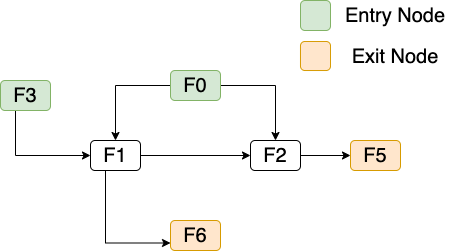
\includegraphics[width=3in]{figures/background/call graph.png}
	\caption{A sample call graph}\label{fig:bg_call_graph}		
	\end{subfigure}
	\quad
	\begin{subfigure}[h]{3in}
		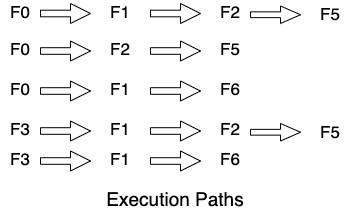
\includegraphics[width=3in]{figures/background/execution_paths.png}
		\caption{All execution paths from the call graph}\label{fig:bg_execution_path}
	\end{subfigure}
	\caption{Call graph with entry node, exit node and execution paths}\label{fig:1}
\end{figure}

An \emph{entry node} for a call graph is the nodes which number of incoming degree is zero. In Figure \ref{fig:bg_call_graph}, the call graph has two entry nodes \emph{F0, F3}. No other nodes call the functions or nodes \emph{F0, F3}. That means program execution can start from this nodes.

An \emph{exit node} for a call graph is the nodes which number of outgoing degree is zero. In Figure \ref{fig:bg_call_graph}, the call graph has two exit nodes \emph{F0, F3}. The exit nodes \emph{F0, F3} do not call any other functions or nodes. That means program execution will end when we come to this node.


The \emph{execution paths} of a call graph are the all possible program execution scenarios. A program execution scenario consist of a function call sequence starting from a \emph{entry node} and ending to a \emph{exit node} of the call graph. In Figure \ref{fig:bg_execution_path}, all the execution paths from the call graph of Figure \ref{fig:bg_call_graph} are listed. First node of the execution paths are the Entry nodes which is defined above. Similarly, Last node of the execution paths are the Exit nodes. 




% \section{Concept Cluster Tree}
% Explain the concept cluster tree, with the role of leaf node, intermediate nodes for example. 


\section{Information Retrieval Techniques}
\subsection{TFIDF}
TFIDF is weight based statistical information retrieval technique. It tries to find important terms to a specific document by analyzing collection of documents. TFIDF is popular for document classification, search engine ranking and text mining\footnote{https://en.wikipedia.org/wiki/Tf–idf}. TFIDF ranks terms by term frequency-inverse document frequency score. Term frequency is count of a term in a document. Term frequency is biased towards common terms which mostly irrelevant to the document. 

\begin{equation}
    tf (W_x, D_x) = f_{W_x,D_x}
    \label{eq:tf_background}
\end{equation}
\begin{equation}
    idf(W_x) = \log(\frac{n}{df(W_x)})+1
    \label{eq:idf_background}
\end{equation}
\begin{equation}
    tf-idf(W_x, D_x) = tf(W_x,D_x) * idf(W_x)
    \label{eq:TFIDF_background}
\end{equation}


Jones \cite{jones1972statistical} introduced inverse document frequency which penalties common terms by counting their occurrence across the corpus. Let, $D = \{D_1, D_2, ..., D_n\}$ is a collection of documents and $W = \{W_1, W_2, ....., W_n\}$ is unique terms in the collection of documents. Now, to calculate term frequency for term $W_x$ in document $D_x$, we have to count frequency of term $W_x$ in  document $D_x$ which is required to calculate term frequency according to equation \ref{eq:tf_background}. In addition, we have to count the number of documents has term $W_x$ which is used to calculate inverse document frequency using equation \ref{eq:idf_background}. In equation \ref{eq:idf_background}, $n$ is the number of documents in the corpus and $df(W_x)$ is the number of documents which contain term $W_x$. Equation \ref{eq:TFIDF_background}, multiplies term frequency and inverse document frequency to reward significant terms and penalize common terms. 



\subsection{LSI}
Latent semantic indexing focuses on information retrieval based on semantic similarity between words where the previous techniques focus on matching words in query with words of documents. The semantic concept used in LSI assumes semantically similar words appear together. Information retrieval techniques which matches words suffer two limitations. They are \emph{synonymy} and \emph{polysemy}. \emph{synonymy} is the issue where same object is described by different words depending on needs, knowledge and linguistic habits. On the other hand, \emph{polysemy} is referred to the fact that words have multiple distinct meaning in different context. LSI, first, starts with Term-Document matrix where all terms are presented in the row and documents in the column. Table \ref{tb:LSI_term_document} shows an example of Term-Document matrix. 

\begin{table}[h]
    \centering
    \caption{Sample Term-Document matrix}
 \begin{tabular}{|c|c|c|c|c|c|c|}
    \hline
    
        & ship & boat & ocean & voyage & trip   \\
        \hline
        Document 1 & 1 & 0 & 1 & 0 & 0  \\
        Document 2 & 0 & 1 & 0 & 1 & 0    \\
        Document 3 & 1 & 0 & 0 & 1 & 1  \\
    \hline
    \end{tabular}
    
    \label{tb:LSI_term_document}
\end{table}


Term-Document matrix is projected to lower number of dimensions by Single Value Decomposition (SVD) method. The reduced matrix by SVD is approximation of the term-document matrix which is a representation of the semantic similarity between words in documents. If we need to find similarity between a query, the query is converted to similar representation and compared to find relevant documents. By using this technique, LSI can detect semantic similarity although the terms are different.   

% \subsection{LDA}

\section{Jaccard Distance}
Jaccard Distance can measure similarity between two sequences according to equation \ref{eq:jaccard}. For example, we have two execution path $E_i$ and $E_j$ and they have set of function names $F_i$ and $F_j$ respectively. Therefore, similarity between $E_i$ and $E_j$ can be measured by equation \ref{eq:jaccard}. 
\begin{equation}
\label{eq:jaccard_similar}
    JD\_similar(E_i, E_j) =  \frac{F_i \bigcap F_j}{F_i \bigcup F_j}
\end{equation}

\begin{equation}
\label{eq:jaccard_dissimilar}
    JD\_dissimilar(E_i, E_j) =  1 - \frac{F_i \bigcap F_j}{F_i \bigcup F_j}
\end{equation}
If $E_i$ and $E_j$ are very similar, according to equation \ref{eq:jaccard_similar} similarity score will be near 1 and vice-versa. Clustering algorithm merges those two clusters which distance measures are minimum. Equation \ref{eq:jaccard_dissimilar} subtract Jaccard Distance by 1 to get desire dissimilarity measure for clustering algorithms.

\section{Agglomerative Hierarchical Clustering}
Clustering algorithms are popular in many data mining, unsupervised machine learning and pattern recognition applications. Clustering algorithm try to group similar observations together to find significant patterns in the observations. Hierarchical clustering can be done in two ways. One is bottom-up (agglomerative) and another is top-down (devisive). For Devisive clustering, all observations starts in a single cluster and divided into different clusters using heuristics. Agglomerative clustering starts by considering observations as individual clusters and then group them until all observations end-up in the same cluster.

\begin{figure*}[h]
  \centering
  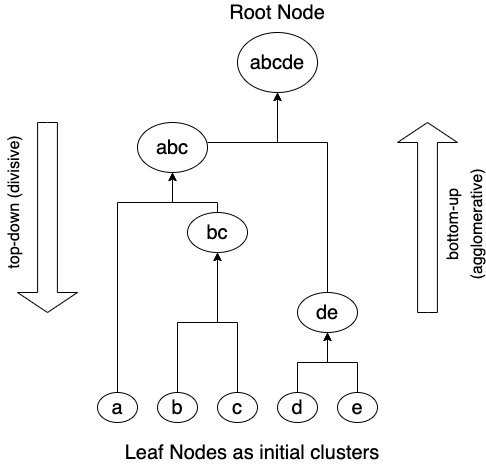
\includegraphics[width=0.5\columnwidth, height=0.5\columnwidth]{figures/background/agglomerative_clustering.png}
  \caption{Agglomerative and Divisive clustering algorithm with a sample cluster forest}~\label{fig:agglomerative_clustering}
\end{figure*}
In Figure \ref{fig:agglomerative_clustering}, a visualization of how agglomerative and divisive clustering algorithm works are presented. Lets assume there are five observations \emph{a, b, c, d, e} and we have similarity score between all the pairs of the observations. First, we can see five observations are treated as five clusters. From the similarity score we found that clusters \emph{d and e} are most similar. Therefore, we group cluster \emph{d and e} together as a new cluster \emph{de}. Now, in the cluster forest we have four clusters. In the next step, cluster b and c are the most similar. So, agglomerative clustering algorithm will group cluster b and c as a new cluster \emph{bc}. The agglomerative clustering will continue to merge clusters together until there is only one cluster in the cluster forest. For this example, the final cluster \emph{(abcde)} consists of all the initial clusters. 

\section{Text Rank}
Mihalcea \cite{mihalcea2004textrank} proposed graph based ranking algorithm inspired by PageRank algorithm to rank entities in natural language. Two of the significant application of TextRank are keyword extraction and sentence extraction. Sentence extraction can be formulated to generate summary of natural language text. To generate summary of a  text, first, sentences are split as they are the unit for TextRank algorithm. Next, sentences are converted to word embedding vectors. In the next step, similarity matrix is computed from embedding vectors. Then, a graph is created where vertices are sentences and edges represent similarity scores between sentences\footnote{https://www.analyticsvidhya.com/blog/2018/11/introduction-text-summarization-textrank-python/}. Similarity scores are used to extract top ranked sentences according to equation \ref{eq:textrank}.

\begin{equation}
\label{eq:textrank}
    WS(V_i) = (1 - d) + d * \sum_{V_j\epsilon IN(V_i) } \frac{w_{ji}}{\sum_{V_k \epsilon Out(V_j)} w_{jk}}  WS(V_j)
\end{equation}

Let, $ G = (V, E)$ is a directed graph where V is the collection of vertices and E is the collection of edges. $In(V_i)$ is the set of vertices which points to vertex $V_i$. Similarly, $Out(V_j)$ is the set of vertices which vertex $V_j$ points to. The similarity score between vertex $V_i$ and $V_j$ is represented by $w_{ji}$. 

% \section{Pyramid Score}

% \section{Sequential Pattern Mining}






% \chapter{Related Work}
% 
\section{Program Comprehension in general}
Program comprehension is a cognitive way of understanding software systems to perform different software maintenance tasks \cite{wei2002surveyCategorizationComprehension, siegmund2016programPastFuture}. Three different type of cognitive models \cite{tilley1998reverseEngineeringFramework, von1993programToolRequirements, siegmund2016programPastFuture} can be found in the literature which is followed consciously or unconsciously by developers. The comprehension models are Top-down, Bottom-up, and Integrated. When developers have prior domain knowledge about a software system, the top-down model is preferred as they can map domain knowledge to low-level source code hierarchically \cite{brooks1983theoryComprehensionPrograms}. On the other hand, when developers lack domain knowledge, they start with low-level source code and then group the functionality together to have a hierarchical abstraction of the system features \cite{shneiderman1979syntacticInteractionsModel, pennington1987stimulusMentalRepresentations}. Integrated model \cite{shaft1995relevanceDomainKnowledge, von1993programToolRequirements} is a mix of top-down and bottom-up approach. The problem in hand and the target system have different properties in the real world, which demand switching between top-down and bottom-up models. Generally, a developer can have prior domain knowledge of a few portion and point-blank for the rest of the system. This situation deserves the adapted use of both top-down and bottom-up approaches.   


\section{IR techniques to Name source code artifacts}
% \cite{mcburney2014improvingTopicSummarize}
% \cite{de2012IRMethodsArtifacts} \cite{panichella2013topicModelsTasks}
% \cite{chen2016topicMiningRepositories}
% Very very important \cite{sun2016surveyTopicSE}
As software repositories contain unstructured data, topic model techniques are widely applied for different software engineering tasks to retrieve information \cite{chen2016topicMiningRepositories, panichella2013topicModelsTasks, sun2016surveyTopicSE}. Most common tasks where topic models showed promising results are source code comprehension, feature location, refactoring, bug localization, and others \cite{sun2016surveyTopicSE}. Lucia et al. \cite{de2012IRMethodsArtifacts} conducted a study to see how information retrieval techniques perform compared to manual naming Java class files. Developers were asked to pick ten keywords for each class file, and top-10 words are picked using different topic model technique and custom heuristics. Their experiment shows that in 40\%-80\% cases, automatic and human label overlaps. 

\section{Reverse Engineering}

\subsection{Subsystem Identification}
Muller et al. \cite{muller1990composingSubsystemStructures} proposed subsystem detection algorithm using different clustering components like variable, procedure, and modules. 
According to Bass et al. \cite{bass2003softwareArchitecturePractice}, two types of software architecture are useful for understanding a complex software system. They are Conceptual and Concrete architecture. A conceptual architecture provides high-level abstraction skipping the code level details. On the other hand, concrete architecture shows the implementation level information. Roy et al. \cite{roy2008softwareArchitectureRecovery} propose and evaluate a framework for the incremental and iterative application of automated architecture recovery (using SWAG Kit) and architecture analysis (using SAAM.). They showed that the reverse engineering tool cannot recover a deeply understood conceptual architecture without SAAM's application but can create a reasonable basis towards that direction. Murphy et al.\cite{MurphyNotkin2001} show that by generating reflexion models from high-level model and source model (i.e., static call graphs), it is possible to facilitate program understanding to the novice developers. 

In this study, we try to automatically recover conceptual architecture from concrete architecture, reducing manual effort.

\subsection{Call graphs to abstract a software system behaviors}
Static and dynamic call graphs are used in literature to help developers comprehend a software system to aid different maintenance tasks \cite{feng2018hierarchicalExecutionComprehension, gharibi2018automaticStaticCluster, xin2019identifyingFeaturesExecution}. Feng et al. \cite{feng2018hierarchicalExecutionComprehension} proposed an approach to use dynamic call graphs for understanding a system's behavior. They instrumented the subject systems to generate execution traces of method entry and exit events. Later, they followed the duplication removal process and constructed a call graph from the execution traces. Execution phases from this dynamic call graph are clustered to get system behaviors. Similarly, Gharib et al. \cite{gharibi2018automaticStaticCluster}, and Vijay et al. \cite{walunj2019graphevoEvolutionCall} also adopted clustering of execution paths from call graphs of the static variant. Using a static call graph brings the benefit of capturing all possible scenarios and less redundant data to handle than dynamic call graph \cite{gharibi2018automaticStaticCluster}. 

\subsection{IR techniques on the hierarchical abstraction of software system}
Feng et al. \cite{feng2018hierarchicalExecutionComprehension} proposed an approach to identify behaviors of a system by hierarchically abstracting dynamic call graph from execution traces. Sequential pattern mining is applied to mine significant portions from the execution phases. Hierarchical clustering is performed to group execution phases. Later, the clusters are labeled using the Tfidf score, where method signatures serve as terms and the phases as document. 
Paul et al. \cite{mcburney2014improvingTopicSummarize} used static call graph to hierarchically abstract a system. In their hierarchical view, each node represents a method. To mine the topics, keywords from methods are considered. Hierarchical Document Topic Model (HDTM) by \cite{weninger2012documentTopicHierarchies} Weninger et al. is adopted, which works on graph documents to mine topic. Gharib et al. \cite{gharibi2018automaticStaticCluster} took a different approach. They went further with the static call graph by extracting execution paths and then clustering the execution paths. Each cluster in the cluster tree is labeled using top-5 method names from Tfidf. Levy et al. \cite{levy2019understandingLargeHierarchical} found interviewing developers that two kinds of comprehension go for large scale hierarchical view. They are system comprehension and code comprehension. In this paper, we tried to adopt static call graph analysis from Gharib et al. and then improve their labeling technique. Nodes of the cluster tree is considered as a behavioral abstraction unit of a system. Method comments are used to generate a description of the unit and sequential pattern mining to create sample examples. 

\section{How developers locate feature on source code}
\textbf{IN PROGRESS}

Include this paper and its related works. \cite{damevski2016field} \cite{kruger2019features} see 5.5.4 process section 

\chapter{ Labeling abstraction nodes and human evaluation}
\label{chapter:hla1}

In this chapter, we discuss different techniques for labeling abstraction nodes and their performance in human evaluation.
Section \ref{approach} presents our approaches for cluster naming, Section \ref{Experimental} describes our experimental design, 
Section \ref{results} presents the technique evaluations, Section \ref{relatedwork} shows the existing approaches,
and finally, Section \ref{conclusion} concludes the paper by mentioning our future direction.  


\section{Introduction}
Understanding the source code of a software system is a prevalent and vital task for the developers because many software engineering tasks depend on program comprehension \cite{cornelissen2009systematic, gilmore1991models, xie2016revisit, feng2018hierarchicalExecutionComprehension}. It is difficult for an individual developer to develop an enterprise software system on their own. Therefore, when someone is assigned to a task or join a development team, they need to understand the existing system to get used to the system. This program comprehension involves a lot of browsing back-and-forth between different granularity levels of the codebase. To reduce developers' effort to comprehend program artifacts, a lot of research is going on in the field of program comprehension \cite{feng2018hierarchicalExecutionComprehension, gharibi2018automaticStaticCluster, kulkarni2014supporting, izu2019program}. An abstract representation of the target software system can easily guide the exploration of low-level source code depending on developers' maintenance tasks. One of the approaches is to generate dynamic logs of function executions while running an existing system on different test cases. The logs can then be used with other methods to produce a suitable output for developers to comprehend the software system \cite{feng2018hierarchicalExecutionComprehension}.
Moreover, most of the dynamic approaches generate dynamic call graphs from the generated dynamic logs of various system scenarios. However, the problem with dynamic call logs is that they only consider the function executions invoked during the dynamic log generation of a target system based on the test cases. As a result, not all the functionalities of the target system are considered during the codebase investigation. Another problem with dynamic logs is that they generate billions of data points, which are mostly redundant. If someone wants to abstract the whole system for comprehension purposes, then using dynamic logs does not help much to cover the entire system.
On the other hand, a static call-graph can be generated by extracting caller-callee relationships from source files. The benefit of a static call graph is that it is possible to have a target system's overall functionalities. The static call graph also resolves the problem of redundant data of the log generations.



A large portion of a developers' development time is devoted to understanding existing source codes \cite{corbi1989program, minelli2015know, ko2006exploratory}. Because without knowing the cognitive relation between source code with higher-level system functionalities, it is difficult to perform different software maintenance tasks (e.g., debugging, feature addition, refactoring, and testing). So, browsing back-and-forth between different source files of a system is widespread among developers to comprehend an existing system. What developers usually do is that they first look for the name of a source file's functions to understand the intention of the functions \cite{de2012IRMethodsArtifacts, starke2009searching}. Therefore, the function names can be utilized for abstracting a system's higher-level functionalities. Moreover, existing studies suggested that \cite{salah2005scenariographerReverseEngineering,pradel2009automaticUseageSpecification} sequence of function invocations can help extract usage scenarios or higher-level functionalities of a target system. Hence, having a tool that visualizes the cognitive mapping between source code and high-level functionalities and allows browsing through source code in a more informed way would help developers.

% \subsection{Why is it hard? (E.g., why do naive approaches fail?)}
% complex source code base, difference between natural language and source code, different characteristics of different language and frameworks, huge amount of data to summarize, creating priority
Manually browsing source code for locating concepts is a laborious task. As a consequence, a lot of existing studies have been done to map concepts with source code using dynamic execution logs. However, very few studies considered static call graphs and emphasized function names. Gharib \textit{et al.} \cite{gharibi2018automaticStaticCluster} proposed a technique based on static call graphs where concepts are mapped with source codes. The authors have presented a whole subject system as a tree where nodes represent concepts of the system. However, they have only applied the TFIDF technique to extract the concepts of a particular codebase. During concept location, they have just considered the name of the function as term. Another drawback of their study is that they have not conducted any use case analysis from users' perspectives. So how developers will be comprehending the source code of a software system is absent in the study for real-world cases.

These limitations of the existing work motivated us to investigate more details on the potential of this approach. We have applied one information retrieval technique, TFIDF, and two topic modeling techniques (LDA and LSI). In the previous study \cite{gharibi2018automaticStaticCluster}, the full function name is treated as a term for the TFIDF technique. Here, we introduce words in function names as another variation. In total, we have six techniques to evaluate, as each technique mentioned above has two variations (function name and words in function name) result. We have also performed a small scale user-study with five developers. We have used 12 clusters from three subject systems as use cases to evaluate our approaches. Developers have rated the summaries generated by each technique and provided their summary of each use case, which we used to assess our automatic techniques using the Pyramid metric. From our investigation, we have found that automatic labeling using TFIDF for words in method names as term variation has an average of 64\% overlap with manual labeling of participants. LDA and LSI received 37\%, and 23\% overlap accordingly. We have also found that words in function name variants got a minimum of 5\% more rating from developers.

In summary, our contributions are:
\begin{itemize}
  \item We adopted two topic modeling techniques to name nodes of the abstract code summary tree. 
  \item We introduce using words in the function name as a term for information retrieval techniques.
  \item We have conducted small scale user study to evaluate the proposed techniques.
\end{itemize}



\section{Motivational Example}
\label{motive}

This section is presented with a motivational example of real-world scenarios. Suppose Bob joined a new company X as a Junior Software Developer. He needs to work on a software project which is being developed for more than six years. He must have a cognitive mapping between source code artifacts and high-level concepts of the software project, which will boost his integration to the project. To get an understanding of the project, he can use the Call graph of the project, which visualizes functional dependency.

\begin{figure*}[h]
  \centering
  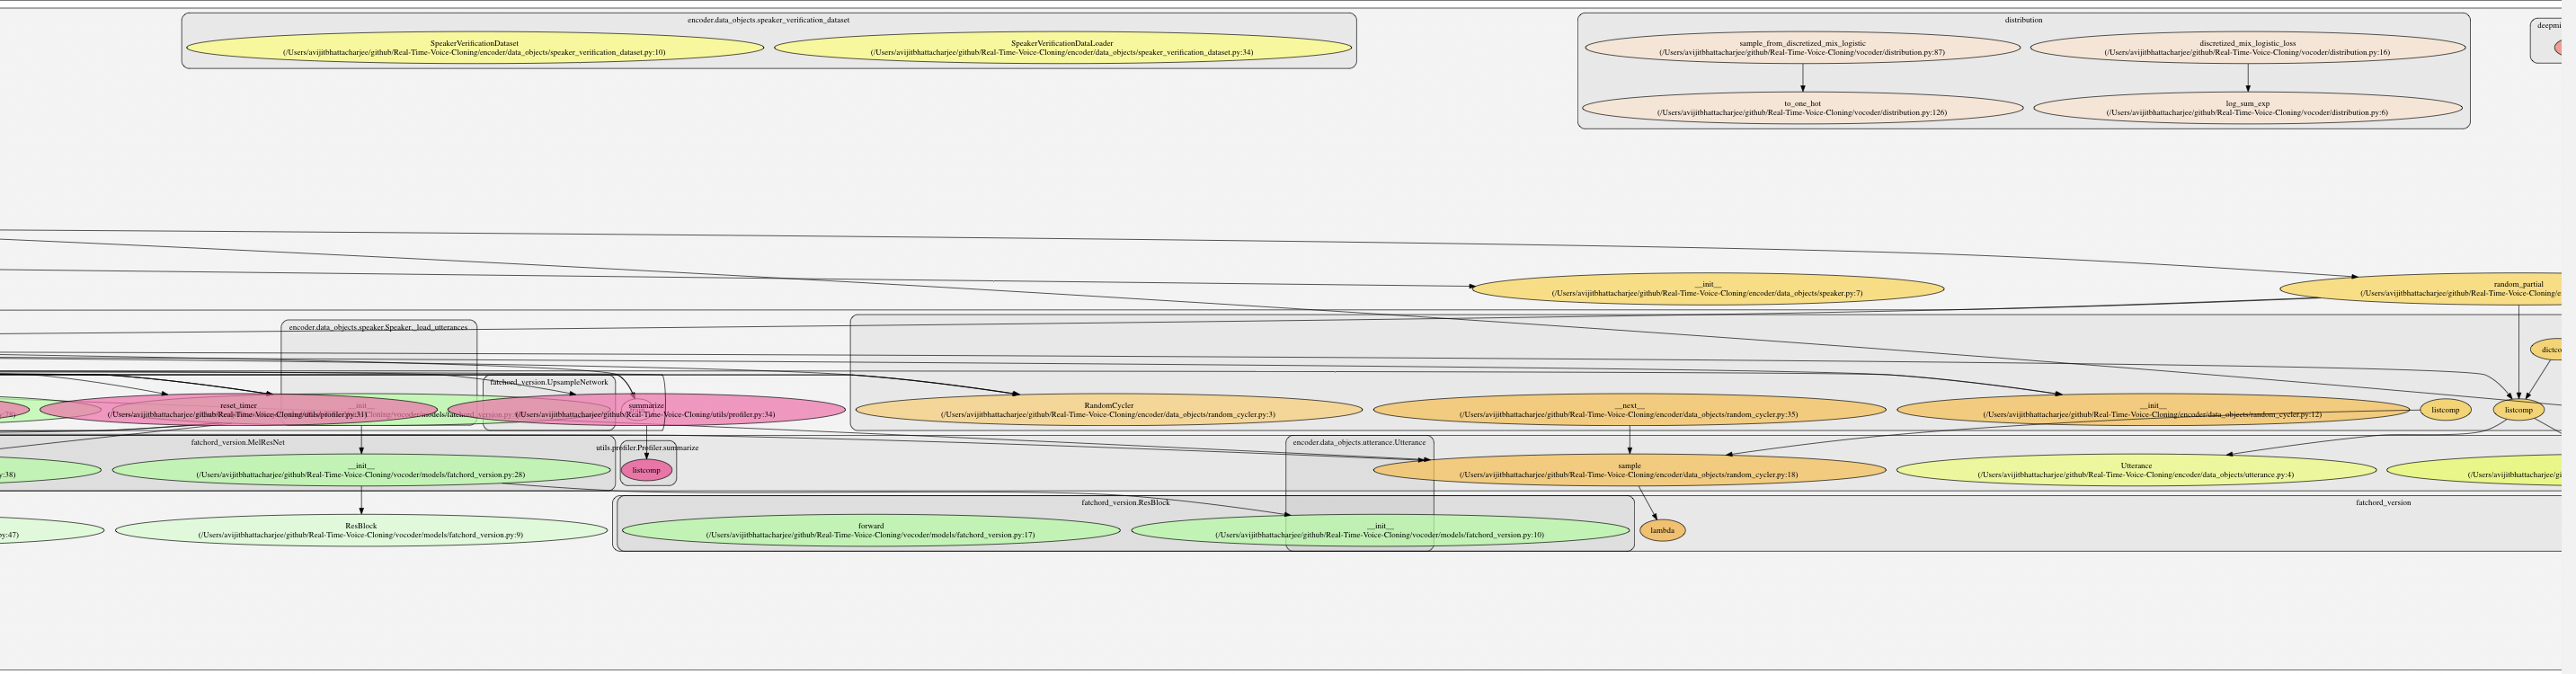
\includegraphics[width=\columnwidth]{figures/hla1/realTime.png}
  \caption{A portion of the Call graph of Real-Time-Voice-Cloning project by Pyan}~\label{fig:realTime}
\end{figure*}

However, in Figure \ref{fig:realTime} we can see a portion of the large call graph generated using Pyan \cite{pyan} for Real-Time-Voice-Cloning \cite{realTime} project. This presentation is very complex and hard to comprehend. Furthermore, if Bob has any particular Software Engineering task to do, first, he needs to locate the concept in source code. Locating source code artifacts relevant to the specific task will help Bob do his task faster. Therefore, our approach starts from this complex call graph and extracts concepts from execution paths in various hierarchical levels. Using the proposed approach, Bob can explore concepts from top-to-bottom, which at the end map to execution paths and the name of functions for smooth inquiries. 


 
 
% \vspace{6mm}
\section{Approach}

\begin{figure*}[tb]
  \centering
  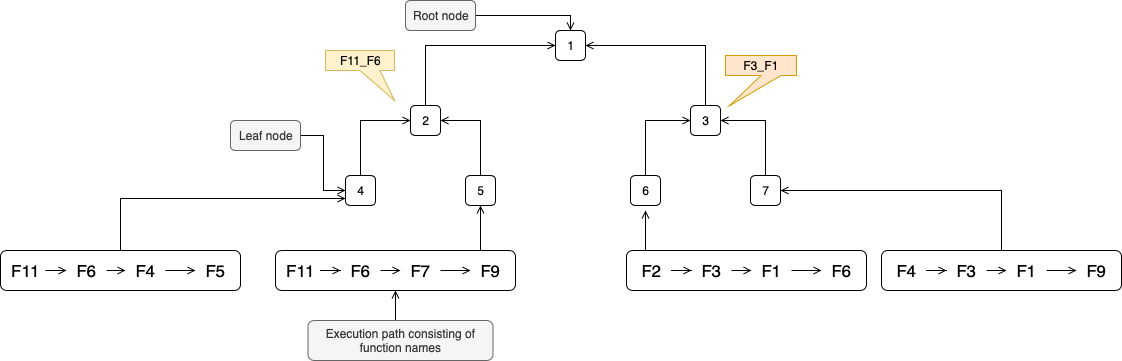
\includegraphics[width=\columnwidth]{figures/hla1/visual_tool_static_call_graph-2.png}
  \caption{Structure of an abstract code summary tree}~\label{fig:hla1_motivation}
\end{figure*}
In this section, we discuss two significant steps in our approach with a brief discussion. First, in Section \ref{hla1:approach_acs}., we described six steps to get the cluster tree of a subject system. Second, in Section \ref{hla1:node_title}, we explain how we used different information retrieval techniques to label nodes of the abstract code summary tree. Data collection for evaluating the approach is depicted in algorithm \ref{hla1:alg:overall}.

\label{approach}

\begin{algorithm}
    \SetKwInOut{Input}{Input}
    \SetKwInOut{Output}{Output}
    
    \underline{Call Graph to abstract code summary tree} $(call graph)$\;
    
    \Input{Call graph}
    \Output{Abstract code summary tree}
    \For{Iterate each node in the call graph}
    {
        \If{ $Number\_of\_Incoming\_Degree(node) == 0$}
        {
            entryNodes.append(node);
        }
        \If{$Number\_of\_Outgoing\_Degree(node) == 0$}{
            exitNodes.append(node);
        }
    } 
    \For{$i\gets1$ \KwTo $entryNodes.length$ \KwBy $1$}
    {
        \For{$j\gets1$ \KwTo $exitNodes.length$ \KwBy $1$}
        {
            execution\_paths.append($simple\_DFS\_path(i, j)$)
        }
    }
    \For{$i\gets1$ \KwTo $execution\_paths.length$ \KwBy $1$}
    {
        \For{$j\gets1$ \KwTo $execution\_paths.length$ \KwBy $1$}
        {
            $distance\_matrix[i][j]$ = $consine\_similarity(i,j)$;
        }
    }
    $cluster\_tree$ = $create\_cluster\_tree(distance\_matrix)$;
    
    $concept\_cluster\_tree$ = $label\_clusters(cluster\_tree)$;
    
    return $concept\_cluster\_tree$;
    \caption{Our procedure for analyzing Python source code of a project to construct an abstract code summary tree}
    \label{hla1:alg:overall}
\end{algorithm}

% \vspace{4mm}
\subsection{Abstract Code Summary (ACS) Tree }
\label{hla1:approach_acs}
The call graph is a visual representation of the relationships between the functions of a project. We adopt static call graphs, which are generated by analyzing source code. As the static call
graphs capture all function calls of a target system, we
choose to abstract the target system. Previous studies suggested that function names contain significant abstraction of source code. Thus, we emphasize mining concepts by analyzing function names in the static call graph.
As we want to capture and abstract the overall system's high-level concepts, therefore, the decision for adopting a static call graph as a building-block of our approach and using function names for concept location is well-justified.  

In Figure \ref{fig:hla1_motivation}, we present the structure of our proposed abstract code summary tree. The leaf nodes of this tree are directly mapped to the execution paths. The execution paths are a list of function names executed sequentially during the execution of a software system. For instance, node 5 is mapped to the execution path where \texttt{ F11, F6, F7, and F9} are called sequentially. Similarly,  in this scenario, all the four-leaf nodes 4, 5, 6, and 7 are mapped to four execution paths or function call sequences. Node 1, 2, and 3 are intermediate nodes of the tree. Naming these intermediate nodes analyzing the execution paths that resides under them might reduce the need to go through in detail about their functionalities. In the figure, node 2 has been named \texttt{F11\_F6}, and node 3 has been named as \texttt{F3\_F1}  by analyzing the function names in the execution paths under those nodes. If we find a proper naming technique that can map concepts in source code with different granularity levels, this approach can make developers program comprehension tasks more flexible. In Figure \ref{hla1:fig:overall}, all the steps are visualized to generate ACS tree from source code.
  

\begin{figure*}[tb]
  \centering
  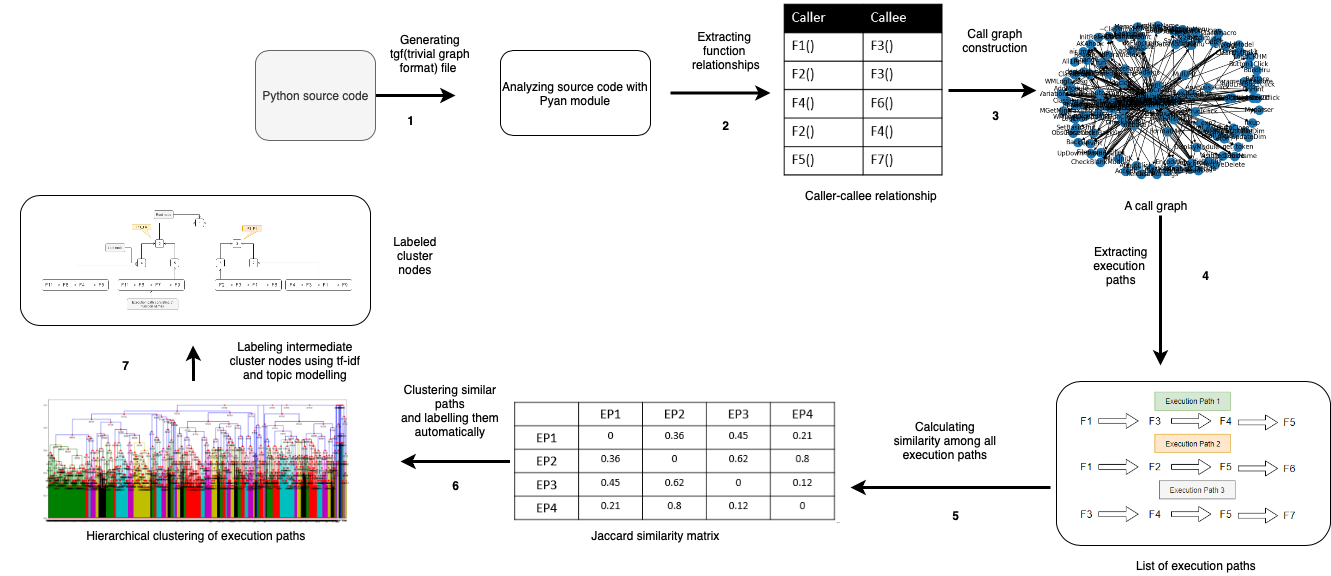
\includegraphics[width=\columnwidth]{figures/hla1/visual_tool_static_call_graph.png}
  \caption{Overview of the overall approach}~\label{hla1:fig:overall}
\end{figure*}

\subsubsection{Analyzing source code using modified Pyan module}

For extracting function relationships from a python system, we used a modified version of Python module Pyan \cite{pyan}. Pyan works only for a single directory. We adapted Pyan so that it can consider multiple directories while extracting the relationships. Pyan uses the abstract syntax tree (AST) for extracting function relationships. After analyzing the source code, we generated a graph in TGF (Trivial Graph Format). In TGF, all modules and functions' physical addresses in the source code are printed first. Then, relationships between all functions are presented as the caller and callee pair.

\subsubsection{Extracting function relationships from TGF}

Function relationships from the TGF file are used as inputs in our technique. Encoded unique identifiers are used to replace function names for ease of processing during the hierarchical clustering step.

\subsubsection{Static call graph creation based on the extracted relationships}
To perform different graph operations, we have created graph objects of the NetworkX \cite{networkx} module using the extracted function relationships. 
\subsubsection{Extracting execution paths}

The execution path is a simple path between an entry node and an exit node. An entry node is a node in the call graph which incoming edge degree is zero. Hence, no function is dependant on an entry node. An exit node is a node that has a zero degree of outgoing function calls. We have generated a list of entry and exit nodes to generate execution paths from a call graph. A simple path means no repeated node visit while visiting from the source node to the destination node. We have collected all possible simple paths for all possible combinations of entry node and exit node pairs. We have implemented a simple path finding algorithm from the NetworkX library, which uses a modified DFS algorithm for finding simple paths between a pair of nodes \cite{networkx}. For our task, a source node is an entry node, and a destination node is an exit node.    

\subsubsection{Distance matrix for execution paths}

For clustering execution paths (sequence of function names), we need to measure the similarity between all pairs of execution paths. For this purpose, we implemented the Jaccard similarity measure \cite{niwattanakul2013jaccardKeywordsSimilarity}. The linkage algorithm uses this similarity in the next step. If we have two sets $ A $ and $ B $, then their Jaccard similarity will be the ratio of their intersection's cardinality by the union. The clustering algorithms work on the distance, which is, in our case, the dissimilarity between two execution paths/clusters. We have subtracted the similarity score with one to get the dissimilarity value according to equation \ref{eq:jaccard}. After calculating dissimilarity between all pairs of execution paths, we converted the 2d matrix to 1d condensed matrix to make our program memory efficient.

\begin{equation}
Dis(A, B) = 1 - \frac{A\cap B}{A\cup B}
\label{eq:jaccard}
\end{equation}

\subsubsection{Clustering execution paths using linkage algorithms}

To group similar execution paths as clusters, we have implemented a linkage algorithm using popular python package Scipy \cite{scipy}. Scipy has different types of linkage algorithms already implemented in its core. To update the distance between two clusters, we have picked Ward the minimum variance method \cite{ward}. Equation \ref{eq:ward} shows how distance using the Ward method is updated when two clusters from cluster forest are merged into a new one \cite{scipy}.

\begin{equation}
     d(u, z) =   \sqrt{\frac{(n_x+n_z)d(x,z)^2+ (n_y+n_z)d(y,z)^2 - n_z d(x,y)^2 }{n_x+n_y+n_z}}
    \label{eq:ward}
\end{equation}

 
In equation \ref{eq:ward}, $u$ is a newly formed cluster, and $z$ is an unused cluster which will be used as reference to calculate distance. $n_x$, $n_y$ and $n_z$ are respectively the number of execution paths (as we are clustering the execution paths) in cluster $x$, $y$ and $z$.
When a new cluster $u$ is created, the distance between $u$ and all the other clusters are updated in the distance matrix. Additionally, cluster $x$ and $y$ are removed from the distance matrix as they have been merged as a new cluster $u$. This step is followed iteratively until only a single cluster remains in the cluster forest. 

For example, in Figure \ref{fig:motivation}, initially, at the start of the clustering process, there are four clusters 4, 5, 6, 7. Next, the hierarchical clustering algorithm selects the two most similar clusters (4, 5 ) to merge them as a new cluster 2. Now, in the clustering process, we have three clusters 2, 6, 7. Similar to the previous step, the most two similar clusters are merged into one. This process continues until there is only one cluster left. Ward method is used to calculate distance between the newly merged cluster with others.

% \vspace{4mm}
\subsection{Naming nodes in an abstract code summary tree}
\label{hla1:node_title}
After getting a cluster tree from the previous step, our next step is to name the clusters to represent the high-level functionality of source code in a readable way. In this step, we will be able to locate high-level concepts in the ACS tree. However, each cluster has a list of function call sequences, and the function call sequences are called execution paths. Our challenge is to extract essential keywords from this collection so that developers can get an overview of the underlying high-level functionalities under the cluster. Naming the source artifacts correctly, in our case, which is nodes in the abstract code summary tree, is the fundamental contribution of this work. Proper naming can help developers to comprehend a program promptly. Toward the naming, we have applied three popular techniques used widely in natural language summarization tasks. These methods try to find meaningful and significant topics from a set of documents. In our approach, a document is an execution path that contains a list of function names. All the execution paths under a cluster are considered as documents.
A previous study used function names as terms in a document \cite{gharibi2018automaticStaticCluster}. However, we want to see what happens if we parse the function names and use the words in function names and use them as a term in documents. We used both words in a function name, and method names approach for the three techniques. Below we briefly described how these three techniques work. 

\subsubsection{TFIDF}
TFIDF \cite{ramos2003usingTfidfRelevance} is a very popular information retrieval technique widely used in text-based search engines. The full form of the TFIDF is term frequency-inverse document frequency. Term frequency means how frequent a term in a document is. Term frequency is calculated according to equation \ref{eq:tf}.

\begin{equation}
    tf(t,d) = f_{t,d}
    \label{eq:tf}
\end{equation}
\begin{equation}
    idf(t) = \log(\frac{n}{df(t)})+1
    \label{eq:idf}
\end{equation}
\begin{equation}
    tf-idf(t,d) = tf(t,d) * idf(t)
    \label{eq:TFIDF}
\end{equation}
The function $f_{t,d}$ counts frequency of term $t$ in the document $d$. Inverse document frequency is calculated according to equation \ref{eq:idf}. Function $df(t)$ in equation \ref{eq:idf} is the count of documents term $t$ is present. The main purpose of $idf$ is to penalize common keywords in the corpus. Term frequency (tf) and Inverse document frequencies (idf) are multiplied to get score for terms. We have adopted \texttt{TFIDFVectorizer} class of scikit-learn \cite{scikit-learn} library for implementing $TFIDF$ technique.
\subsubsection{LDA}
Latent Dirichlet Allocation (LDA) \cite{blei2003latentLDA} is a statistical model that tries to describe a set of documents by assuming they are created from some topics. LDA is a very popular topic modeling technique. LDA assumes every term in a document belongs to some topic. So, it assumes each term belongs to some topic and then performs analysis to find which assumptions are supported by statistics of the corpus. We have used Gensim \cite{gensim} library for implementing LDA for our approach.
\subsubsection{LSI}
Latent Semantic Indexing (LSI) \cite{deerwester1990indexingLSI} is a technique used in natural language processing. LSI assumes semantically similar words occur together. First, the term-document frequency matrix is calculated from the corpus. Then, this term-document frequency matrix is decomposed into three matrices using the Single Value Decomposition (SVD) technique. Terms are first assigned to topics using the term-document frequency matrix. Then, using all the topics, a topic importance matrix is derived, which leads to topics for the documents. Similar to LDA, we used Gensim \cite{gensim} library for implementing LSI. 

\section{Experimental Design}
\label{Experimental}
This section will discuss the research questions that need to be answered regarding the abstract code summary tree, how we collected our subject systems for the experiment, and details about users who participated in this study.
% \vspace{4mm}
\subsection{Research questions}
We want to explore how manual naming supports automatic naming techniques. To investigate this, we set \texttt{RQ1}.
Besides, we have compared developer preferences for three different techniques using function names as terms by \texttt{RQ2}. Similarly, for \texttt{RQ3}, we changed the input for information retrieval techniques by words in function names instead of function names and compared developers' ratings among the three approaches. Finally, we want to see the performances of our two variations of choosing terms by a systematic comparison by \texttt{RQ4}. 
\begin{itemize}
    
    \item \textbf{\texttt{RQ1}} How well does the automatic labeling perform using the candidate approaches compared to manual labeling?  (To evaluate this, we will use pyramid measure)
    \item \textbf{\texttt{RQ2}} How do developers evaluate different labeling approaches based on function names?
    \item \textbf{\texttt{RQ3}} How do developers evaluate different labeling approaches based on words in method names? 
    \item \textbf{\texttt{RQ4}} How can we compare the preferences of developers between the two approaches addressed in \texttt{RQ2} and \texttt{RQ3}? 
\end{itemize}
% \vspace{4mm}
\subsection{Dataset Collection}

In order to conduct the user-study, we have collected source code of three popular Python projects \texttt{Detectron} \cite{Detectron2018}, \texttt{Real\-Time\-Voice\-Cloning} \cite{realTime} and \texttt{requests}\cite{requests}. The reason behind choosing these subject systems for our study is that they are popular among Python developer communities. These projects follow the standard conventions of software developments so participants will be able to relate keywords from their day-to-day knowledge. Additionally, open-source projects tend to follow proper function naming conventions, which is important for our approach as it completely depends on function names. We extracted source code and applied the steps described in Section \ref{alg:overall}. We have printed clusters with their corresponding execution paths and names suggested by the candidate techniques in a file for doing the user-study. We have chosen 12 clusters semi-randomly, i.e.,  four from each of the subject systems, which ensures the coverage of different levels' clusters. 
% \vspace{4mm}
\subsection{User-study}
\begin{figure*}[h]
    \begin{center}
    \subcaptionbox{Full abstract code summary tree with local view\label{fig:tool_ui}}
    {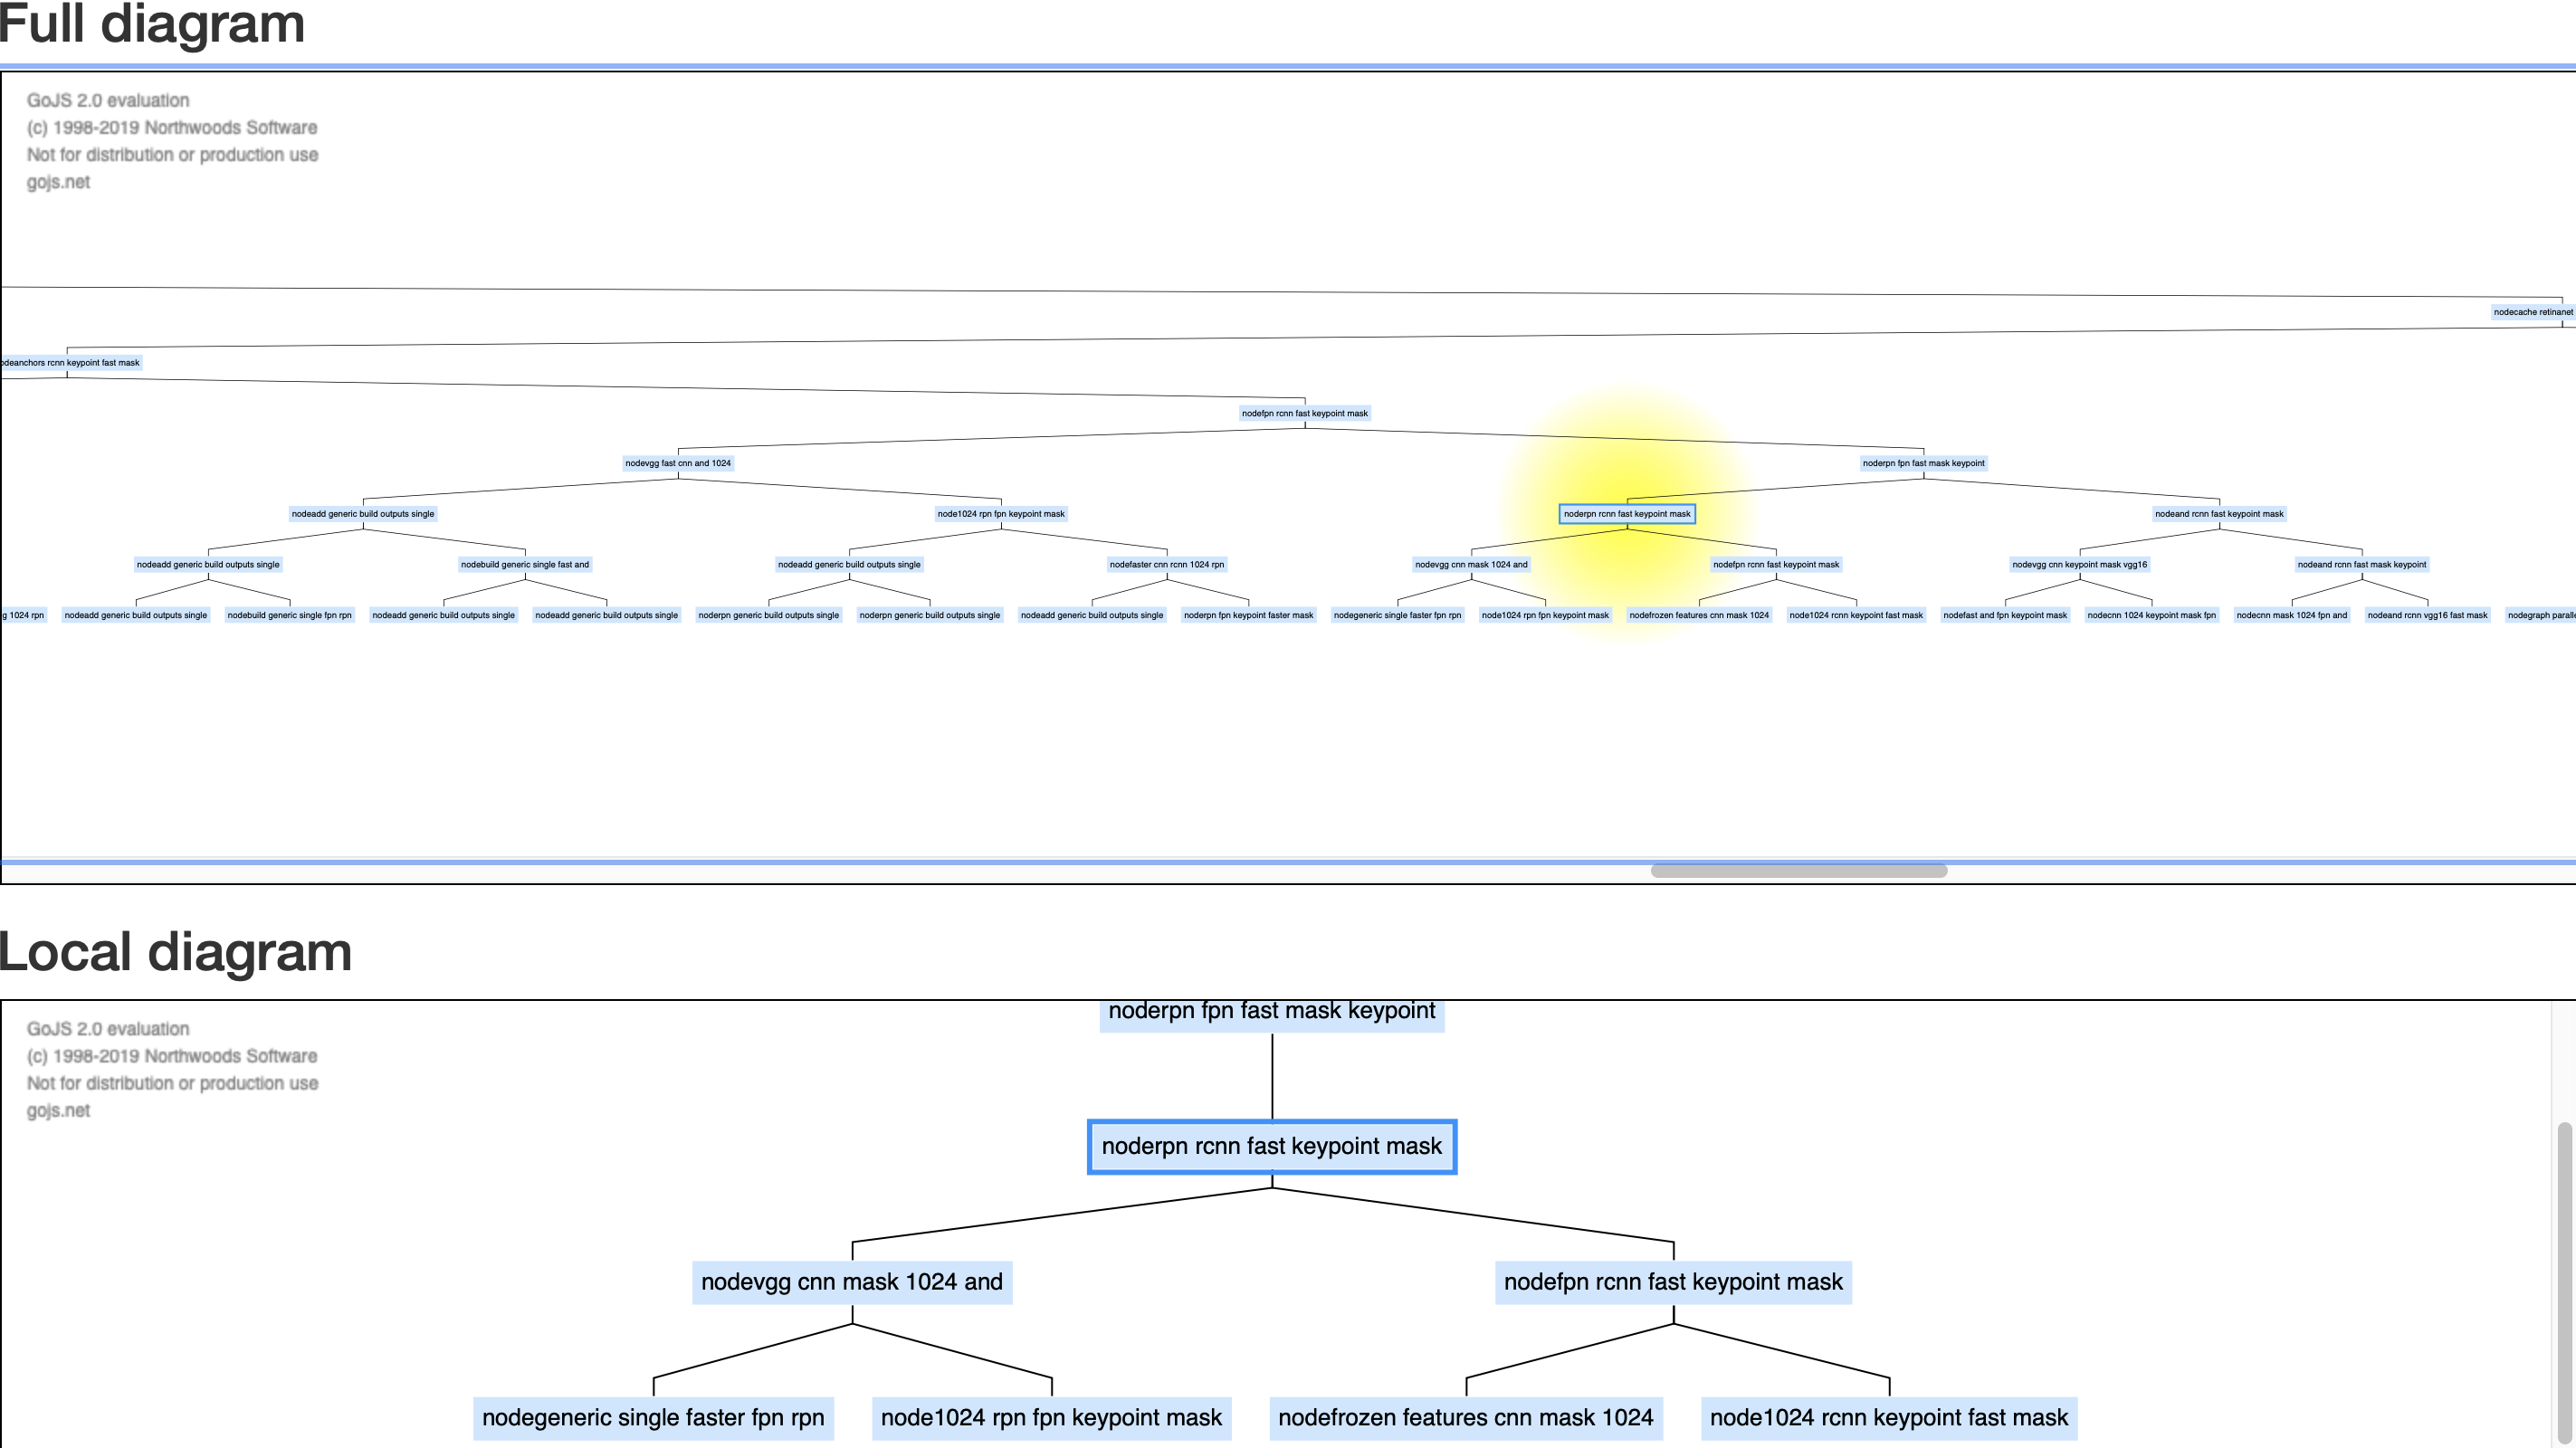
\includegraphics[scale=0.25]{figures/hla1/ToolUI.png}}
    \subcaptionbox{Form presented to the participants for answering\label{fig:userstudy}}
    {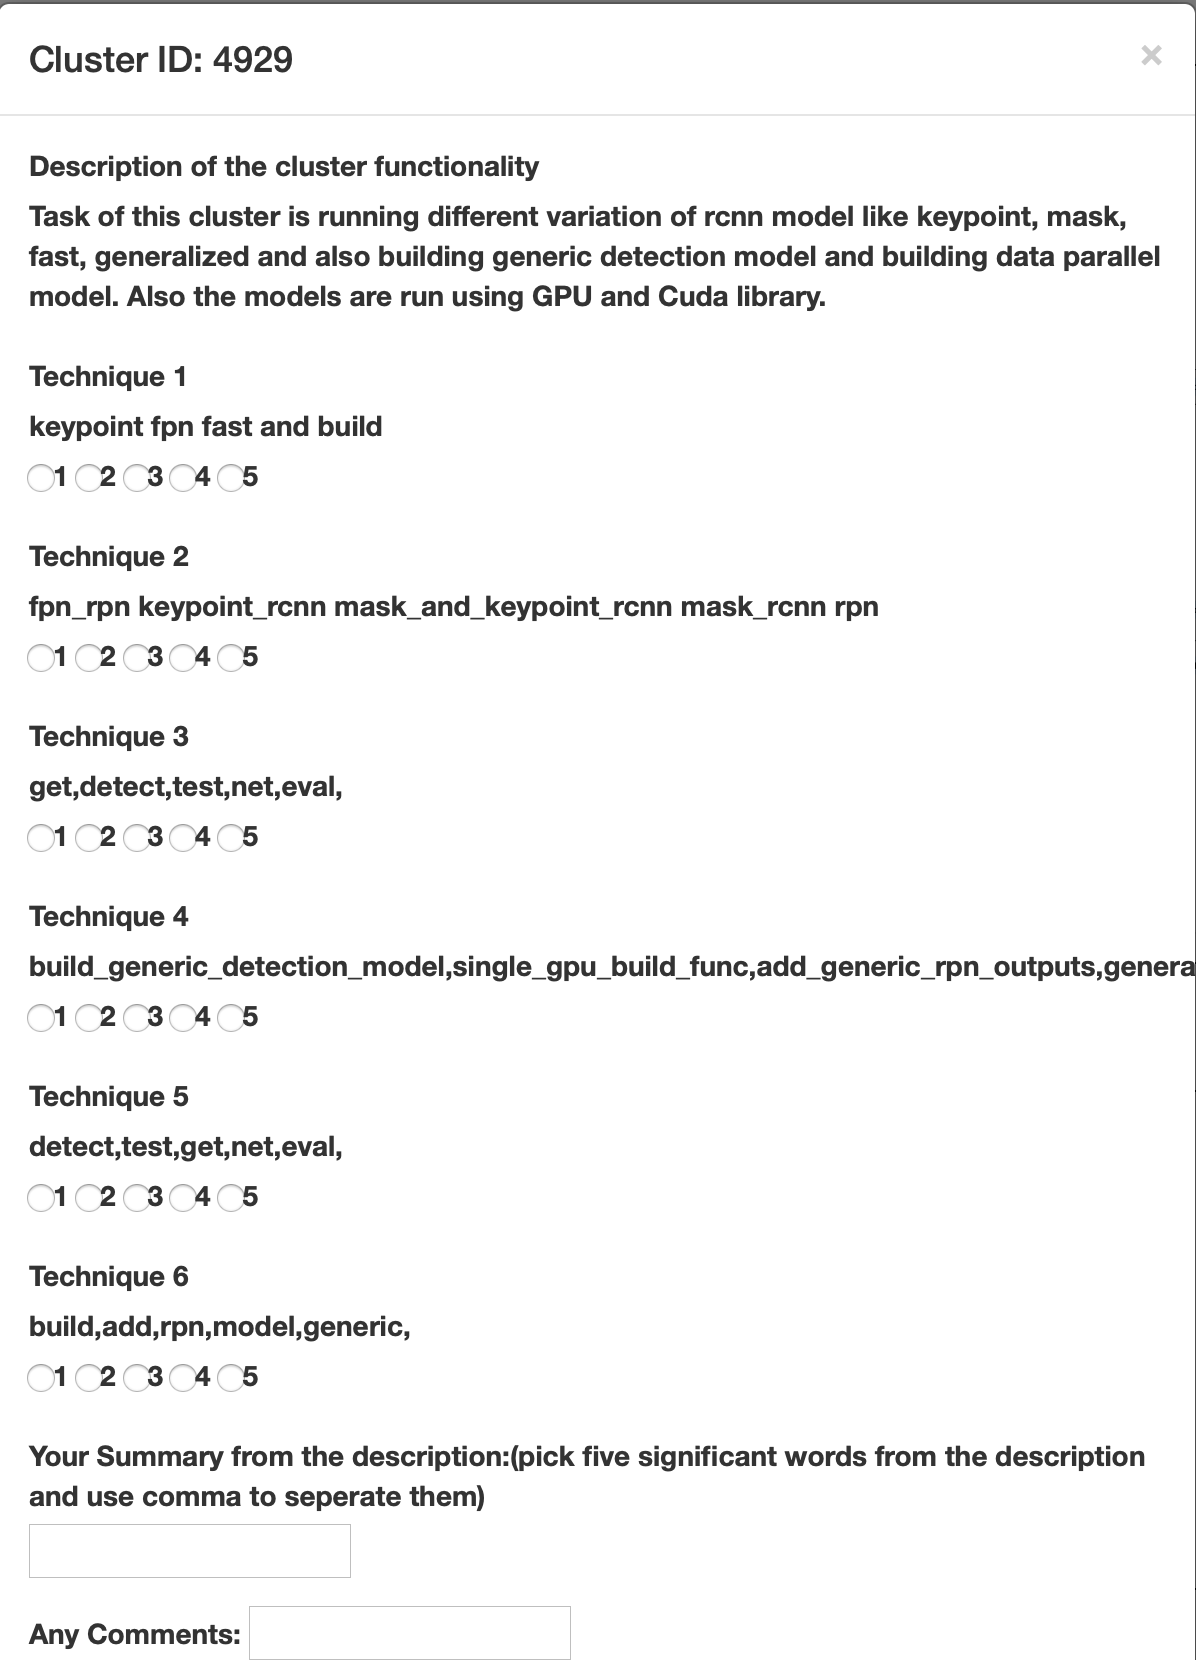
\includegraphics[scale=0.23]{figures/hla1/userstudy.png}}
    \caption{Tool UI presented to the study participants}
    \label{fig:tool}
    \end{center}
    
\end{figure*}
For the 12 clusters, we manually analyzed each cluster's execution paths and come up with a 2-3 line description of what happens inside the clusters. Before the study, we told users to rate the automatic summaries of our three techniques, each with two variations. Additionally, we also provided a text box for the participants to select five keywords from the description produced by manual analysis of execution paths. We have used this summary to compute the Pyramid score for the three techniques of the words in function name variation. A total of five persons participated in the study with a software development background. Among them, three are female, and two are male. Each of the participants has at least a Bachelor's degree in Computer Science. Two of them are graduate students, and the other three are working as developers in three different software firms. All of them have at least three years of experience in programming experience with an average of 3.8 year. 


In Figure \ref{fig:tool_ui}, the abstract code summary tree from our tool is presented. The upper box contains the full abstract code summary tree. Below the concept tree, a local view can be used to look closer to the concept cluster. Developers can click on any node in the concept diagram to get a zoomed view of its child and parents. 

In Figure \ref{fig:userstudy}, a screenshot of the form provided to the participants is presented. When participants right-click on the target clusters, a form with cluster id and a brief description of the execution paths' manual analysis is popped up. In the form, we asked the participants about their preference (1 means least preferred, 5 means most preferred) for names suggested by the six techniques and selected five keywords from the descriptions to complete the study.


\section{Results and Discussion}
\label{results}
% \vspace{3mm}
\subsection{User Naming vs. Automatic Naming}
To investigate how automatic naming accords with manual naming, we have used Pyramid score \cite{nenkova2004evaluating}. Pyramid score is used in natural text summarization tasks to compare an automatic summary with a manual summary. Haiduc et al. \cite{haiduc2010supporting}  used Pyramid score to support source code summary with developers' summary, which motivated us to adopt Pyramid score to find out how our automatic approaches of abstraction harmonize with developers' selections. In Table \ref{table-pyramid1}, we have shown the Pyramid score calculation process for a cluster (i.e., cluster number 10 of the 12 clusters). The preferences of five developers who participated in this study are represented by D1,\ldots, D5. X\_word represents the corresponding outputs of $X \in {TFIDF, LDA, LSI }$ by considering words in function names. Each column presents unique keywords from the selections of five participants. Furthermore, we have marked which words are matched with the automatic summary from a developers' summary in the corresponding cells. In each row for the automatic techniques, we have put the support from five developers for keywords being present in the summary. For example, we can see that keyword $response$ is present in TFIDF with words in the function name variation, and four of the developers picked $response$ in their summary. So, support for keyword $response$ is given 4. To get the Pyramid score for cluster number 10, we have summed each keyword's support in automatic naming by developers. In this case, values are $4(response), 2(send), 1(merge)$. We divide the sum of these support values by the top five most frequent keywords of five developers' summary. So, the score is now $(4+2+1)/(4+4+3+2+2) = 0.466 $ for cluster 10. Greater Pyramid score means that the automatic naming is becoming more human in our case. In Figure \ref{fig:pyramid12}, we have plotted Pyramid score for 12 clusters with the three techniques of word variant and support of the five participants for them. In the figure, we can see that for most of the clusters, the \texttt{TFIDF\_word} based automatic naming technique's summary agrees more compared to other techniques with  the developers' provided summaries.

\begin{table*}[h]
\small
\caption{Pyramid score computation }
\label{table-pyramid1}
\centering
\begin{tabular}{|l|l|l|l|l|l|l|l|l|l|l|l|l|}
\hline
  & response & request &	dict &	send &	from &	build &	cookiejar &	create &	get &	cookie &	prepare &	merge  \\ \hline
D1 & x      & x     & x           & x   & x    &        &         &     &      &    &  &    \\ \hline
D2 &     x   &      &  x       &     &    & x      & x       &   &      & x& &       \\ \hline
D3 & x      &       &           &    &     &    x    &         & x   &  x    & x & &     \\ \hline
D4 &        &       &             &   x  &     &        &        &     & x    & x    & x &    \\ \hline
D5 &  x     &      &    x         &     &     &        &        & x    &     & x    &  &   \\ \hline
\texttt{TFIDF\_word}  &   x(4)     &       &             &  x(2)   &  &        &     &     &  &  & & x(1)    \\ \hline
\texttt{LDA\_word}  &        &   x(1)    &             &     &  &        &     &     & x(2) &   & x(1) &  \\ \hline
\texttt{LSI\_word}  &        &   x(1)    &             &  x(2)   &   &        &  x(1)     &     & x(2) &  & & \\ \hline
\end{tabular}
\end{table*}

\begin{figure*}[h]
 \pgfplotstableread{
 1 0.7857 0.71 0.29
2 0.71 0.29 0.14
3 0.53 0.06 0.06
4 0.56 0.125 0.125
5 0.61 0.46 0.15
6 0.57 0.05 0.315
7 0.9 0.72 0.09
8 0.53 0.53 0.46
9 0.43 0.31 0
10 0.46 0.26 0.4
11 0.81 0.5 0.43
12 0.73 0.4 0.33
}\dataset
% \resizebox{6.0in}{!}{
\begin{tikzpicture} \begin{axis}[xbar,
ylabel={\#Cluster no.},
xlabel={Pyramid score},
 symbolic y coords={1, 2, 3, 4, 5, 6, 7, 8, 9, 10, 11, 12},
        ytick=data,
        nodes near coords, 
        nodes near coords align={horizontal},
        bar width=0.18cm,
width=\textwidth,
% height=7.5cm,
xmin=0,
xmax=1.0, 
xticklabel style={font=\footnotesize},
yticklabel style={font=\footnotesize, /pgf/number format/fixed},
y tick label style={ rotate=0},
major y tick style = {opacity=0},
minor y tick num = 1,
minor tick length=1ex,
xmajorgrids = true,
%grid=both,
%grid style={line width=.1pt, draw=black!10},	
legend entries={TFIDF\_word,LDA\_word, LSI\_word},	
legend style={at={(0.5,-0.1)},
anchor=north,
legend columns=6,
font=\scriptsize,
% text width=2.75in,
% minimum height=0.20in,
nodes near coords
}
        ]
    \addplot [draw=black!100, fill=black!10] table[x index=1,y index=0] \dataset;
    \addplot [draw=black!100, fill=black!30] table[x index=2,y index=0] \dataset;
    \addplot [draw=black!100, fill=black!50] table[x index=3,y index=0] \dataset;
    
\end{axis}
\end{tikzpicture}
% }
  \caption{Pyramid score of the 12 clusters}~\label{fig:pyramid12}
  \vspace{-2mm}
\end{figure*}

% \vspace{3mm}
\subsection{User Rating on Function Name Variant}
To answer the RQ2, we use the techniques with function names as unit variation. We asked our participants to rank each technique's summary with a score ranging from 1 to 5 to reflect how well they support the manual description. In Figure \ref{fig:method}, we have plotted the average ranking of the participants for 12 clusters with the techniques. In the figure, we can see the users preferred LSI naming technique over the LDA. LSI is preferred in almost 50\% of the clusters. For clusters 1, 4, 9, participants' preference for LDA and LSI are the same. The reason is that both techniques provided a similar kind of summary for the cluster in the automatic naming process.

\begin{figure*}[h]
\pgfplotstableread{
 1	2.6	3	3
 2	3.4	2.8	4
 3	2.8	2.8	3.4
 4	3	3.2	3.2
 5	3.2	3	2.6
 6	3.2	2.2	2.8
 7	3.2	2.8	3.2
 8	3.4	2.8	3.2
 9	3.2	3.4	3.4
 10	3	3.4	3.6
 11	3	3.8	3.2
 12	3.6	3.4	3
}\dataset
\resizebox{6.0in}{!}{
\begin{tikzpicture}
\begin{axis}
[ybar,
% enlargelimits=0.05,
bar width=0.10cm,
width=0.55\textwidth,
height=4.5cm,
ymin=0,
ymax=5.0, 
ylabel={Average ranking of
five participants},
xlabel = {\#Cluster no.},
yticklabel style={font=\footnotesize},
xticklabel style={font=\footnotesize, /pgf/number format/fixed},
xtick=data,
xticklabels = {1, 2, 3, 4, 5, 6, 7, 8, 9, 10, 11, 12},
x tick label style={ rotate=45},
major x tick style = {opacity=0},
minor x tick num = 1,
minor tick length=1ex,
ymajorgrids = true,
label style={font=\footnotesize},
%grid=both,
%grid style={line width=.1pt, draw=black!10},	
legend entries={TFIDF(function names),LDA(function names), LSI(function names)
},	
legend style={
at={(0.5,-0.35)},
anchor=north,
legend columns=-1,
font=\scriptsize,
%text width=2.75in, 
minimum height=0.20in,
nodes near coords style={rotate=90,  anchor=west, font=\tiny},
nodes near coords
},
]
% \addplot[draw=black!100, fill=green!20,pattern= grid] table[x index=0,y index=1] \dataset;
\addplot[draw=black!100, fill=black!10] table[x index=0,y index=1] \dataset;
\addplot[draw=black!100, fill=black!30] table[x index=0,y index=2] \dataset;
\addplot[draw=black!100, fill=black!50] table[x index=0,y index=3] \dataset;
\end{axis}
\end{tikzpicture}
}
\caption{User preference among three implemented naming techniques (considering methods as terms)}
\label{fig:method}
% \vspace{-2mm}
\end{figure*}

\begin{figure*}[h!]
\pgfplotstableread{
1	3.4	3.4	3
 2	3.4	3.2	3
 3	3	3.2	2.8
 4	3.2	3	3.2
 5	3.4	3.8	3
 6	3.6	3.4	3.8
 7	3.6	3.6	3.6
 8	3.2	3	3.6
 9	4	3.4	4.2
 10	3.6	3.6	4
 11	3.8	3.6	3.8
 12	3.8	3.8	3.4
}\dataset
\resizebox{6.0in}{!}{
\begin{tikzpicture}
\begin{axis}
[ybar,
% enlargelimits=0.05,
bar width=0.10cm,
width=0.55\textwidth,
height=4.5cm,
ymin=0,
ymax=5.0, 
ylabel={Average ranking of
five participants},
xlabel = {\#Cluster no.},
yticklabel style={font=\footnotesize},
xticklabel style={font=\footnotesize, /pgf/number format/fixed},
xtick=data,
xticklabels = {1, 2, 3, 4, 5, 6, 7, 8, 9, 10, 11, 12},
x tick label style={ rotate=45},
major x tick style = {opacity=0},
minor x tick num = 1,
minor tick length=1ex,
ymajorgrids = true,
label style={font=\footnotesize},
%grid=both,
%grid style={line width=.1pt, draw=black!10},	
legend entries={TFIDF(words in function names),LDA(words in function names), LSI(words in function names)
},	
legend style={
at={(0.5,-0.35)},
anchor=north,
legend columns=-1,
font=\scriptsize,
% text width=2.75in,
minimum height=0.20in,
nodes near coords style={rotate=90,  anchor=west, font=\tiny},
nodes near coords
},
]
\addplot[draw=black!100, fill=black!10] table[x index=0,y index=1] \dataset;
\addplot[draw=black!100, fill=black!30] table[x index=0,y index=2] \dataset;
\addplot[draw=black!100, fill=black!50] table[x index=0,y index=3] \dataset;
\end{axis}
\end{tikzpicture}
}
\caption{User preference among three implemented naming techniques (considering words in methods as terms)}
\label{fig:word}
\vspace{-2mm}
\end{figure*}

\begin{figure*}[h]
  \pgfplotstableread{
  

  1 3.5 3.133333333
  2 3.416666667 3.05
  3 3.45 3.216666667
}\dataset
\begin{tikzpicture}
\begin{axis}[xbar,
bar width=0.50cm,
% ylabel={\#Cluster no.},
% xlabel={Pyramid score},
yticklabel style={font=\footnotesize},
xticklabel style={font=\footnotesize, /pgf/number format/fixed},
xmin = 0,
xmax = 5.0,
yticklabels = {TFIDF, LDA, LSI},
%  symbolic y coords={TFIDF, LDA, LSI},
        ytick=data,
        legend entries={words\_in\_function\_names, function\_names},	
         nodes near coords, 
        nodes near coords align={horizontal},
legend style={
at={(0.5,-0.15)},
anchor=north,
legend columns=-1,
font=\scriptsize,
%text width=2.75in,
minimum height=0.20in}
]
    \addplot [draw=blue,
        pattern=horizontal lines ,
    ] table[x index=1,y index=0] \dataset;
    \addplot [draw=green,
        pattern=crosshatch ,
    ] table[x index=2,y index=0] \dataset;
\end{axis}
\end{tikzpicture}
  \caption{Comparison between three techniques considering function names and words in function names}~\label{fig:method_vs_word}
\end{figure*}

\subsection{User Rating on Words in Function Name Variant}
We have followed a similar approach to answer RQ3 that we used to answer RQ2. We averaged five participants' rankings for 12 clusters for the three techniques (TFIDF, LDA, LSI). In RQ3, we want to know participants' preference when we consider words in the function names as unit for the TFIDF, LDA, LSI-based techniques. In Figure \ref{fig:word}, we have plotted user rankings of the automatically suggested names for 12 clusters. Among twelve clusters, we can see that in seven of them, developers preferred names suggested by TFIDF and LSI technique in preference to the LDA technique, which covers almost 60\% of the clusters. Therefore, \texttt{RQ3} can be answered to establish that words in function name variation perform better with TFIDF, LSI than LDA.      



\subsection{Function Name vs. Words in Function Name}
For \texttt{RQ4}, we want to see users' preference on TFIDF, LDA, and LSI based techniques of the two variations we mentioned in \texttt{RQ2} and \texttt{RQ3}.
So, we averaged the user rankings of 12 clusters of three techniques from Figure \ref{fig:method} and Figure \ref{fig:word}. In Figure \ref{fig:method_vs_word}, we plotted the average ranks of the three techniques in two variations (i.e.,function\_names and  words\_in\_function\_names). From the figure, we can observe that developers preferred TFIDF, LDA, and LSI techniques with word as unit over method name variations. Words in function names variation get at least 5\% higher preference than the method names variations for each of the three techniques. 

\section{Related Work}
\label{relatedwork}
Feng \textit{et al.} \cite{feng2018hierarchicalExecutionComprehension} proposed an approach to abstract execution traces for program comprehension. To get execution traces, they used BLINKY to instrument source code for getting method-invocation calls. Different test cases are used to generate execution traces for different scenarios. From dynamic logs, they have built phase trees that are created from caller-callee relationships of invoked methods. After deleting duplicate phases, they clustered unique phases using the Agglomerative hierarchical clustering algorithm. Next, they applied a mining technique to get frequent pattern phases of each level of clustered phase tree. For comprehension purposes, they used TFIDF to rank method names of frequent phases and then used the top 20 method names for the final label. Depending on dynamic call graphs comes with some limitations as it depends on the test cases heavily, and the size of log file generated is difficult to handle. Therefore, we choose static call graphs to remove the test dependency and capture a call graph's overall execution scenario. Gharib \textit{et al.}  \cite{gharibi2018automaticStaticCluster} proposed an approach using static call graphs for hierarchical abstraction. First, they generated a static call graph for a subject system that captures overall function relationships. Second, execution paths from the call graph are extracted, which become the building blocks for their approach. Next, execution paths are clustered together to create abstract code summary of the target subject systems. Feng \textit{et al.}~\cite{feng2018hierarchicalExecutionComprehension} also named the clusters by extracting keywords from the function names present in execution paths. In their study, only the TFIDF technique is applied to extract and name intermediate clusters.

For this study, our motivation is to take forward this approach and enrich it with existing techniques from the literature. Two limitations of the study from Gharib \textit{et al.}  are using only TFIDF method for information retrieval and no presence of user study to validate how developers prefer the output abstractions. We adopt two more topic modeling techniques for information retrieval, which show promising results for naming source code artifacts in the literature \cite{de2012IRMethodsArtifacts}. Andrea \textit{et al.}  \cite{de2012IRMethodsArtifacts} tried to apply IR techniques like VSM, LDA, and LSI on  source code artifacts. To evaluate IR techniques' effectiveness, they also produced suggestions from 17 users on the same classes. Then, they assessed the performance of automatic naming by comparing overlap
with manual naming of users. In their study, authors also find that heuristic based approaches focusing on function signatures perform well for code artifacts summarization. Inspired from their study, we use LDA and LSI on function signatures to extract concepts in code in this paper. Another improvement from Gharib \textit{et al.} is to adopt a user study for validating automatic abstraction. Sonia \textit{et al.}  \cite{haiduc2010supporting} used Pyramid score to evaluate the output of automatic code summary with developers' summary. We also adopt this Pyramid score, which is widely used for the evaluation of natural language summaries. 

\section{Threats to Validity}
We have used three subject systems for the user study, and all of them are written with the Python language. We acknowledge that our user sample size is small. To mitigate the effect of randomness, we used three different systems, considered four clusters from each of them and invited experienced developers for the study. Our approach depends on function names. Therefore, our approach would be less successful when the naming conventions are not properly followed. We have used open-source projects which generally maintain good naming conventions.  We have collected user summary after they evaluated six techniques to understand the limitation of automatic naming and provide feedback accordingly.  
% \vspace{6mm}
\section{Conclusion and Future Work}
\label{conclusion}
While proposing an approach to find concepts in source code from static call graph analysis, we try to remove the shortcomings of existing approaches in terms of techniques evaluation and use cases. We use two different variations of terms to recommend concepts that leverage developers' program perception effort while understanding a system. As program comprehension is a subjective matter, we collect user data to evaluate how our automatic labeling approach accords with user choice. The techniques we use are TFIDF, LDA, and LSI, with two variations (i. e., naming by function names, and naming by words in function names), where we found the TFIDF works better in cluster naming, and users prefer words in functions variants.   

During our manual analysis to generate a brief description of twelve clusters by observing execution paths, we found patterns in execution paths that might make the naming of concept cluster more human. In the future, we will try to adopt sequential pattern mining techniques to name clusters more meaningfully. Additionally, we plan to build an interactive tool that developers can use to browse concepts in a software system. The current technique is intended to focus on Python-based projects, and we are planning to add support for other languages for the technique.



\chapter{ Providing summary and significant patterns for abstraction nodes}
\label{chapter:hla2}
In this chapter, we briefly discuss how we generated summary and execution patterns for abstraction nodes. Section \ref{hla2:approach} describes how the proposed approach works. In Section \ref{hla2:evaluation}, an exploratory case study is reported to validate our proposed techniques.

% Program comprehension is a concept of understanding code to perform different software maintenance tasks. In recent years, the size of the code base is increasing drastically, which makes program comprehension difficult. To cope with the demand, many research works have been performed to understand how developers comprehend a program or code snippet and how to support developers to start their assigned tasks quickly. Different cognitive models are proposed in the literature to ease comprehension. 
% Recently, studies to cluster execution paths of a call graph to aid overall program comprehension are going on.
% We argue that this structure can be used to aid the top-down and bottom-up cognition model of program comprehension.
% This paper has adopted new techniques for the hierarchical abstraction of a software system that performs better than the existing literature's related techniques. We conducted an exploratory case-study with three subject systems to validate our hypothesis. We found that it is possible to use this hierarchical presentation to enrich above mentioned cognition models.   

\section{Introduction}

One of the crucial parts of a software engineering job is software maintenance. Usually there are four types of software maintenance tasks, such as 
 perfective, preventive, corrective, and adaptive \cite{williams2010characterizingArchitectureChanges}. To perform all of these tasks, developers first need to understand the target system, how its different components work together, and locate the relevant classes, methods, and files for completing a specific task. To add or change something in the system accurately and adequately, developers need to understand how its different components work together and map the implementation level source code to high-level features. Proper tool support for program comprehension can reduce the manual and economic cost of software maintenance, which will result in cheaper software \cite{arisholm2006impactUMLDocumentation}. In the literature, the studies on program comprehension are divided into two parts \cite{levy2019understandingLargeHierarchical}. First, how developers understand a code snippet. Second, understanding how large software systems are comprehended. Levy et al. \cite{levy2019understandingLargeHierarchical} conducted a study to find how comprehending a large system works from an experienced developer's perspective. The comprehension of a system has a conceptual and concrete level \cite{bass2003softwareArchitecturePractice, levy2019understandingLargeHierarchical}. In reverse software engineering, different tools are used to extract implementation level architecture from source code (call graph). Later, through manual analysis, they are mapped to concept level architecture, which helps cognitive mapping \cite{roy2008softwareArchitectureRecovery}. However, as software systems are getting more complex in size, manual analysis of implementation level architecture to high-level concepts requires more human resources. In most cases, they are exhausting. 

Studies \cite{cornelissen2007understandingMassiveSequence, feng2018hierarchicalExecutionComprehension, reiss2005dynamicSoftwarePhases, watanabe2008featurePhaseDetection} on processing call graphs to facilitate overall system comprehension are very common in literature. The dynamic call graph is used for most studies, which is appropriate for specific test cases or scenarios. The problem with the dynamic call graph is they have redundancy problems and cannot capture the whole software systems \cite{gharibi2018automaticStaticCluster}. Recently research on overall system comprehension focused on static call graph took attention \cite{gharibi2018automaticStaticCluster, walunj2019graphevoEvolutionCall}. Execution paths from static call graphs \cite{pradel2009automaticUseageSpecification, salah2005scenariographerReverseEngineering} can be used to extract usage scenario or high level functionality. Clustering execution paths from both static and dynamic call graph pave the way for the abstract code summary of the system \cite{feng2018hierarchicalExecutionComprehension, gharibi2018automaticStaticCluster}. We argue that labeling nodes of an abstraction tree  can aid developers in using different program comprehension models. For example, the Bottom-up model is used by developers when they do not have any knowledge about the domain of the system. They gradually try to map low-level properties to high-level concepts. Developers can use the cluster tree of execution paths to facilitate Bottom-up cognition. The clustering starts from execution paths (low-level features) to a gradual grouping of similar paths, which are high-level features. Similarly, the abstraction tree can help automate the top-down cognition model. 

In the top-down model, when developers have domain knowledge of a system, they try to map the knowledge to low-level implementations. The cluster tree hierarchically abstracts the features so that we have domain knowledge at the top of the tree that we can relate to low-level features by browsing the tree in a top-down manner. From our manual investigation to the proposed approach of Gharib et al. \cite{gharibi2018automaticStaticCluster}, we found that the abstraction tree has the potential to support program comprehension models automatically. However, they only used top-5 function names from the execution paths as the abstraction node label. We found that labeling the abstraction node properly with supporting documentation and example can make the abstract code summary tree more attractive and comprehensive to the developers. 
\begin{itemize}
    \item First, we experimented with labeling the nodes using TFIDF, LDA, and LSI information retrieval techniques. Previous studies only used the TFIDF technique.
    \item Second, we generated natural text descriptions for each node by summarizing comments from the execution paths' methods.
    \item Third, inspired by Feng et al. \cite{feng2018hierarchicalExecutionComprehension}, for each node, we attached significant patterns from execution paths by applying Sequential pattern mining. To validate our techniques, we conducted an exploratory case study with three subject systems to find how these techniques can automatically help developers in program comprehension. 
\end{itemize}

Our investigation shows that providing a natural text description and sample execution patterns increase the comprehensibility of abstraction nodes. 

 

\section{Approach}
\label{hla2:approach}
\begin{figure*}[tb]
  \centering
  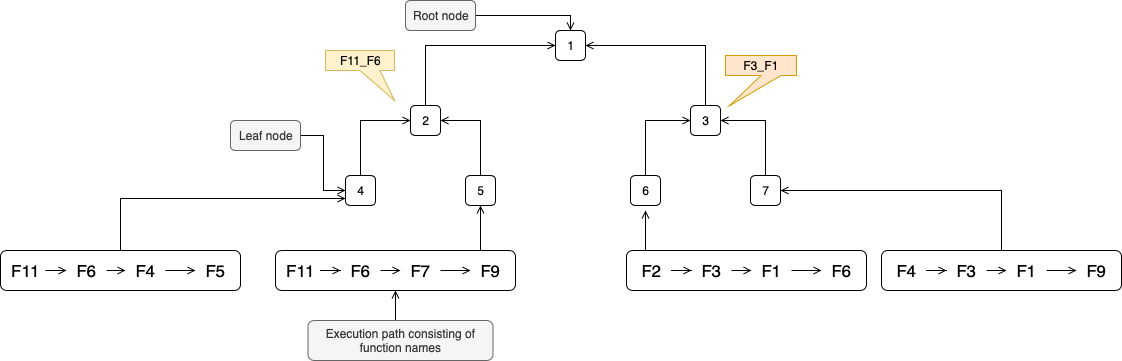
\includegraphics[width=\columnwidth]{figures/hla2/tree_structure.png}
  \caption{Structure of a abstract code summary tree}~\label{fig:tree_structure}
\end{figure*}
In this section, we discuss two significant steps in our approach with a brief discussion. First, we described six steps to get the subject system's abstract code summary tree in Section III-A. Second, in Section III-B, we describe how we used different information retrieval techniques to define the tree's hypothetical abstraction nodes. Data collection for evaluating the approach is depicted in algorithm \ref{alg:overall}.


\begin{algorithm}
    \SetKwInOut{Input}{Input}
    \SetKwInOut{Output}{Output}
    
    \underline{Call Graph to abstract code summary tree} $(call graph)$\;
    
    \Input{Call graph}
    \Output{Abstract code summary tree}
    \For{Iterate each node in the call graph}
    {
        \If{ $Number\_of\_Incoming\_Degree(node) == 0$}
        {
            entryNodes.append(node);
        }
        \If{$Number\_of\_Outgoing\_Degree(node) == 0$}{
            exitNodes.append(node);
        }
    } 
    \For{$i\gets1$ \KwTo $entryNodes.length$ \KwBy $1$}
    {
        \For{$j\gets1$ \KwTo $exitNodes.length$ \KwBy $1$}
        {
            execution\_paths.append($simple\_DFS\_path(i, j)$)
        }
    }
    \For{$i\gets1$ \KwTo $execution\_paths.length$ \KwBy $1$}
    {
        \For{$j\gets1$ \KwTo $execution\_paths.length$ \KwBy $1$}
        {
            $distance\_matrix[i][j]$ = $consine\_similarity(i,j)$;
        }
    }
    $cluster\_tree$ = $create\_cluster\_tree(distance\_matrix)$;
    
    $hierarchical\_abstraction\_tree$ = $label\_clusters(cluster\_tree)$;
    
    return $hierarchical\_abstraction\_tree$;
    \caption{Our procedure for analyzing Python source code of a project to construct abstract code summary tree}
    \label{alg:overall}
\end{algorithm}

% \vspace{4mm}
\subsection{Abstract code summary tree of a software system}
A call graph is a visual representation of a software system's method invocation relationships between different methods. We adopted a static call graph, which is generated by analyzing source code. As a static call graph captures whole function calls of a target system, we choose to abstract the target system. Previous studies suggested that function names contain significant abstraction of source code. 
Thus, we emphasized mining keywords by analyzing function names in the static call graph.
As we wanted to abstract the whole system's high-level functionality hierarchically, therefore the decision to adopt the static call graph as a building-block of our approach is well-justified.

In Figure \ref{fig:tree_structure}, we presented the abstract code summary tree structure. The leaf nodes of this tree are directly mapped to the execution paths. Execution paths are a list of function names executed sequentially during the execution of a software system. For instance, node 5 is mapped to the execution path where F11, F6, F7, and F9 are called sequentially. 
In this scenario, all the leaf nodes (4, 5, 6, 7) are mapped to four execution paths or function call sequences.
Node 1, 2, and 3 are hypothetical abstractions of the four leaf nodes.
Generating meaningful descriptions for these intermediate nodes can make the abstraction tree helpful towards different program comprehension cognition models.
In the figure, nodes 2, 3 have been labeled F11\_F6, F3\_F1, respectively. These labels are generated by analyzing their child nodes' function names. We plan to generate five keywords for each intermediate node, alongside a short natural text description (from the doc-string of function names) and few significant patterns from analyzing execution paths under investigation.

\begin{figure*}[tb]
  \centering
  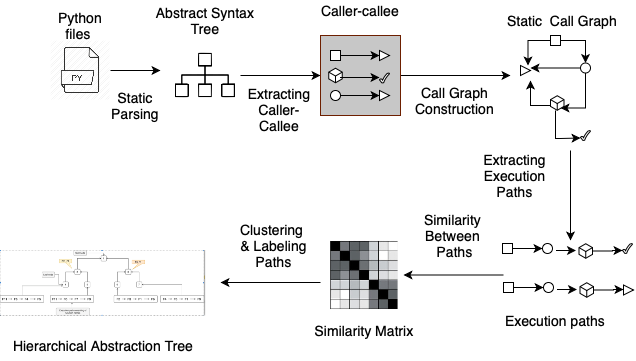
\includegraphics[width=\columnwidth]{figures/hla2/approach_new.png}
  \caption{Overview of the overall approach}~\label{fig:overall}
\end{figure*}

\subsubsection{Analyzing source code using modified Pyan module}

We used a modified version of Python module Pyan \cite{pyan} to extract function relationships from a Python system. Pyan works only for a single directory. We adapted Pyan so that it can consider multiple directories while extracting the relationships. Pyan uses the AST tree for extracting function relationships. After analyzing the source code, we generated a graph in TGF format (Trivial Graph Format). In TGF format, all modules and functions' physical addresses in the source code are printed first. Then, relationships between all functions are presented as the caller and callee pair.

\subsubsection{Extracting function relationships from Trivial graph format}

Function relationships from the TGF file format are used as inputs in our technique. Encoded unique identifiers are used to replace function names for ease of processing during the hierarchical clustering step.

\subsubsection{Static call graph creation based on the extracted relationships}
To perform different graph operations, we have created graph objects of NetworkX \cite{networkx} module using the extracted function relationships. 
\subsubsection{Extracting execution paths}

The execution path is a simple path between an entry node and an exit node. An entry node is a node in the call graph which incoming edge degree is zero. So, no function is dependant on an entry node. An exit node is a node that has a zero degree of outgoing function calls. We have generated a list of entry and exit nodes to generate execution paths from a call graph. Simple Paths calculation algorithm of the NetworkX \cite{networkx}  is used in our approach, which applies the \texttt{DFS} algorithm to get the paths between a source node and a destination node. For our task, a source node is an entry node, and a destination node is an exit node.    

\subsubsection{Distance matrix for execution paths}

For clustering execution paths (sequence of function names), we need to measure the similarity between all pairs of execution paths. For this purpose, we  \cite{niwattanakul2013jaccardKeywordsSimilarity} implemented the Jaccard similarity measure. The linkage algorithm uses this similarity in the next step. If we have two sets $A$ and $B$, then their Jaccard similarity will be the ratio of the cardinality of their intersection by the union. As clustering algorithm works on distance in our case dissimilarity between two execution paths/clusters, we have subtracted the similarity score with one to get the dissimilarity value according to equation \ref{eq:jaccard}. After calculating dissimilarity between all pairs of execution paths, we converted the 2d matrix to 1d condensed matrix to make our program memory efficient.

\begin{equation}
Dis(A, B) = 1 - \frac{A\cap B}{A\cup B}
\label{eq:jaccard}
\end{equation}

\subsubsection{Clustering execution paths using linkage algorithms}

To group similar execution paths as clusters, we have implemented a linkage algorithm using the popular Python package Scipy \cite{scipy}. Scipy has a lot of different types of linkage algorithms already implemented in its core. To update the distance between two clusters, we have picked the Ward \cite{ward} minimum variance method. Equation \ref{eq:ward} \cite{scipy} shows how distance using the Ward method is updated when two clusters from cluster forest are merged into a new one.

\begin{equation}
     d(u, z) =   \sqrt{\frac{(n_x+n_z)d(x,z)^2+ (n_y+n_z)d(y,z)^2 - n_z d(x,y)^2 }{n_x+n_y+n_z}}
    \label{eq:ward}
\end{equation}

 
In equation \ref{eq:ward}, $u$ is a newly formed cluster, and $z$ is an unused cluster which will be used as reference to calculate distance. $n_x$, $n_y$ and $n_z$ are respectively the number of execution paths (as we are clustering the execution paths) in cluster $x$, $y$ and $z$.
When a new cluster $u$ is created, the distance between $u$ and all the other clusters are updated in the distance matrix. Additionally, cluster $x$ and $y$ are removed from the distance matrix as they have been merged as a new cluster $u$. This step is followed iteratively until only a single cluster remains in the cluster forest. 

% \vspace{4mm}
\subsection{Generating summary for the intermediate abstraction nodes}
After getting a tree by clustering execution paths in the previous step,  
we generate three types of summaries for each intermediate node. First, we used different 
information retrieval techniques like TFIDF, LDA, and LSI for selecting five keywords or five function names from analyzing execution paths descendant to an intermediate node. This information is the label of the intermediate nodes. Second, this time instead of considering the function names, we considered the function names' comments to provide natural text summary for each intermediate node. Comments from the functions are summarized using TextRank \cite{barrios2016variationsTextRankSummarization} algorithm. Given a collection of sentences as input, this algorithm can summarize the collection to a fixed number of sentences. Third, inspired by Feng et al. \cite{feng2018hierarchicalExecutionComprehension}, to provide a glimpse of the significant patterns among execution paths SPAM (sequential pattern mining) algorithm PrefixSpan \cite{han2001prefixspanSequentialPatterns} is implemented. We find that all the execution paths in an intermediate node share some patterns from our manual investigation of the execution paths. By taking a look at the significant patterns, we can comprehend more elaborately about the intermediate nodes. We present these patterns in support of the Label and Summary generated by the previous two steps. Therefore, to comprehend an abstraction node, we have a label, summary description, and patterns from the execution paths. Below we briefly described the steps. 

\subsubsection{Label intermediate/abstraction nodes}
\begin{itemize}
    \item TFIDF:
TFIDF \cite{ramos2003usingTfidfRelevance} is a very popular information retrieval technique widely used in text-based search engines. The full form of the TFIDF is term frequency-inverse document frequency. Term frequency means how frequent a term in a document is. Term frequency is calculated according to equation \ref{eq:tf}.

\begin{equation}
    tf = f_{t,d}
    \label{eq:tf}
\end{equation}
\begin{equation}
    idf = \log(\frac{n}{df(t)})+1
    \label{eq:idf}
\end{equation}
\begin{equation}
    tf-idf(t,d) = tf(t,d) * idf(t)
    \label{eq:TFIDF}
\end{equation}
The function $f_{t,d}$ counts frequency of term $t$ in the document $d$. Inverse document frequency is calculated according to equation \ref{eq:idf}. Function $df(t)$ in equation \ref{eq:idf} is the count of documents term $t$ is present. The main purpose of $idf$ is to penalize common keywords in the corpus. Term frequency (tf) and Inverse document frequencies (idf) are multiplied to get score for terms. We have adopted \texttt{TFIDFVectorizer} class of scikit-learn \cite{scikit-learn} library for implementing $TFIDF$ technique.
    \item LDA:
Latent Dirichlet Allocation (LDA) \cite{blei2003latentLDA} is a statistical model that tries to describe a set of documents by assuming they are created from some topics. LDA is a popular topic modeling technique. LDA assumes every term in a document belongs to some topic. So, it considers each term belongs to some topic and then performs analysis to find which assumptions are supported by statistics of the corpus. We have used Gensim \cite{gensim} library for implementing LDA for our approach.
    \item LSI:
Latent Semantic Indexing (LSI) \cite{deerwester1990indexingLSI} is a technique used in natural language processing. LSI assumes semantically similar words occur together. First, the term-document frequency matrix is calculated from the corpus. This term-document frequency matrix is decomposed into three matrices using the Single Value Decomposition (SVD) technique. Terms are first assigned to topics using the term-document frequency matrix. Then, using all the topics, a topic importance matrix is derived, which leads to topics for the documents. Similar to LDA, we used Gensim \cite{gensim} library for implementing LSI. 
\end{itemize}

\subsubsection{Summary description of intermediate/abstraction node}
To generate a summary for node 3 of Figure \ref{fig:tree_structure}, we collect the first line of docstring comment for the function F1, F2, F3, F4, F6, F9 as they consist of the execution paths of node 3's descendant nodes. Next, we remove duplicates from the comments and provide these sentences to TextRank \cite{barrios2016variationsTextRankSummarization} algorithm to generate summary. There are many functions in an execution path for real-world software, so using the TextRank algorithm, we get a short five sentence comprehensive summary. 

TextRank~\cite{barrios2016variationsTextRankSummarization} is a graph-based automatic summarization technique. TextRank is language and domain-independent. To generate a summary, training a corpus is not required, making it suitable for our task. All the sentences of the target document make the nodes of a graph. Edges between the nodes are created using different similarity measures between two nodes or sentences. At last, PageRank~\cite{page1999pagerank} algorithm is used to obtain a summary from the graph.

\subsubsection{Significant patterns for intermediate/abstraction node}
To get significant patterns for node 3 in Figure \ref{fig:tree_structure}, we have to analyze execution paths of node 6 and node 7. The execution paths of node 6 and 7 have $ F3 \rightarrow  F1 $ sequence common. So, presenting this common sequence as a significant pattern for node 3 make a good abstraction of descendant execution paths of node 3. To mine this sequential patterns, we implement PrefixSpan \cite{han2001prefixspanSequentialPatterns} sequential pattern mining algorithm. If we provide a collection of execution paths to PrefixSpan, it gives a significant pattern analyzing the collections. PrefixSpan creates a prefixed based projection database to find sequential patterns efficiently.

\section{Experimental Design}
\label{hla2:evaluation}
This section will discuss research questions that drive this study, how we collected our subject systems, what criteria were considered, and how we designed our exploratory case study. 

\subsection{Research Questions}
In this paper, we tried to improve the comprehensiveness of the abstraction of nodes. First, we split function names to get words so that TFIDF, LDA, and LSI methods perform naturally. There is also another benefit of using words in method names as they will be fixed length. We investigate how effective node names are using the word variant in our RQ1. Besides, we attach a natural text summary for each node using the docstring of functions, which consists of RQ2. Similarly, we generate significant patterns from execution paths to support node comprehension, and this is our RQ3. Finally, we investigate how merging the results of RQ1, RQ2, and RQ3 improves the abstraction tree in RQ4. 

\begin{itemize}
    
    \item \textbf{\texttt{RQ1}} How effective is the word variation of TFIDF compared to method variation?
    \item \textbf{\texttt{RQ2}} How comprehensive is the natural text summary for abstraction nodes?
    \item \textbf{\texttt{RQ3}} How effective are the mined patterns to comprehend abstraction nodes?
    \item \textbf{\texttt{RQ4}} How effective is the comprehension of an abstraction node, if label, summary, and patterns are used together?
\end{itemize}

\subsection{Dataset Collection}
In this study, we have experimented with three subject systems. We cloned the source code of the subject systems from their Github repository. We used the Pyan library to extract caller-callee relationships in trivial graph format (TGF). Next, we created a networkX graph object to iterate through the call graph and extract execution paths. Finally, the Ward linkage clustering algorithm was used to create an abstract code summary tree. In table \ref{table:subject_systems}, we present the entry, exit nodes, line of code, number of execution paths. We chose our subject systems carefully to have three different execution paths as the number of execution paths determines how big the abstraction tree will be. We wanted to keep the size manageable for performing our analysis to find our proposed techniques' effectiveness. 

\subsection{Case Study Design}
To find the effectiveness of the proposed techniques, we carefully chose different abstraction nodes and their neighbourhood. After that, we manually checked whether the label, summary and mined patterns suitably abstract and describe the system's high-level concepts. To verify whether the approaches properly support our claim, we manually browsed the source code of target systems to know the systems' high-level concepts. To generalize our findings to some extent, we have used three different subject systems so that our claim is stronger.

\begin{table*}% put at top of page if possible 
 \caption{3 Subject Systems with their No. Entry, Exit Nodes, LOC, Paths, And Date Retrieved}
\centering
% \resizebox{3.4in}{!}{
\begin{tabular}{l|l|l|l|l|l|l|l}
No & URL & Name & Entry Nodes & Exit Nodes & LOC & Paths & Date retrieved\\
 & (https://github.com) &  &  &   & & &\\
\hline
1 & \url{Our code}& higher\_level\_abstraction & 2 & 22 & 999 & 31 &  28 May 2020\\
2 & \url{/davidfraser/pyan} & pyan & 36 & 50 & 3711 & 637 & 28 May 2020\\
3 & \url{/CorentinJ/Real-Time-Voice-Cloning}& Real-Time-Voice-Cloning & 21 & 93 & 9117 & 404 & 28 May 2020\\


\end{tabular}
% }
\label{table:subject_systems}
\end{table*}

\section{An Exploratory Case-study}
\begin{figure*}[tb]
  \centering
  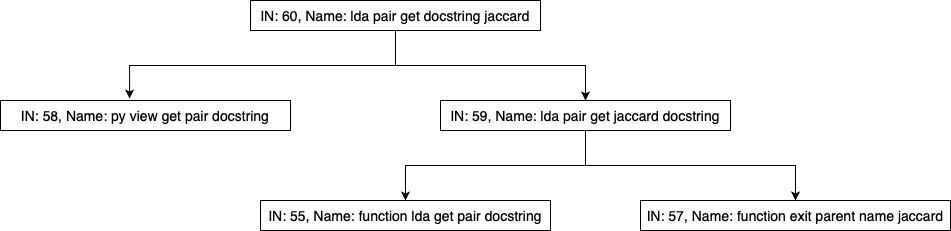
\includegraphics[width=1\columnwidth]{figures/hla2/rq1_hla1.png}
  \caption{Snippet from subject system 1 (Our code)}~\label{fig:rq1_hla1}
\end{figure*}

\subsection{ RQ1: Effectiveness of Word Variation Labeling}
To see the effectiveness of labelling, we manually picked the root node and its neighbourhood. We explored a similar tree snippet for the three systems. In Figure \ref{fig:rq1_hla1}, we see root node 60 has the label \textit{lda pair get docstring jaccard}. From this label, one can guess that something related to docstring, Jaccard distance, and topic modelling LDA occurs in the higher\_level\_abstraction subject system. An interesting thing to notice is that name of node 60 and 59 is the same. Although node 58 is a child node of 60, which has two new keywords py and view that indicate something related to Python file and view occurs inside the nodes' execution paths. On the other hand, if we see the name for node 60 using TFIDF method variant ( \textit{pretty\_print\_leaf\_node bfs\_with\_parent mining\_sequential\_patterns id\_to\_sentence cluster\_view}), we see that using method as unit for TFIDF is more comprehensible than using word as unit for TFIDF. Another benefit of TFIDF method variant is for node 60 and 59; it provides different names according to their execution paths. On the other side, the word variant of TFIDF gives the same name for nodes 60 and 59 because of over\-fitting.

\begin{figure*}[tb]
  \centering
  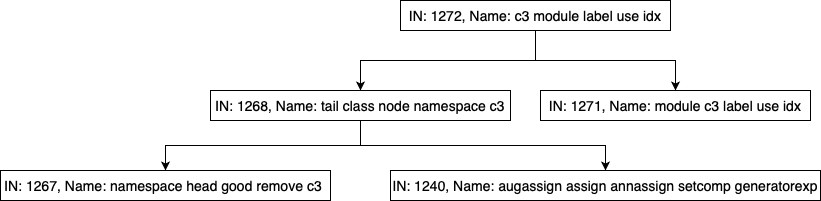
\includegraphics[width=\columnwidth]{figures/hla2/rq1_pyan1.png}
  \caption{Snippet from subject system 2 (pyan)}~\label{fig:rq1_pyan1}
\end{figure*}

In figure \ref{fig:rq1_pyan1} shows that we have a snippet of the Pyan subject system's abstraction tree. Pyan~\cite{pyan} is an open-source software which can extract call graph from a Python project. From our general knowledge, we can expect the concepts related to source code. If we look at node 1272 at Figure \ref{fig:rq1_pyan1}, the name is \textit{c3 module label use idx}. Except for the module, other keywords are not that much expressive. For node 1268, we see keywords like class, node, namespace indicate that the node is relevant to processing source code. However, we can see a recurrent occurrence of the same name for nodes 1272, 1271, which is an over-fit situation. The names for nodes 1272, 1271 using method variant TFIDF are \textit{write\_edge  find\_filenames  DotWriter}, \textit{write\_edge TgfWriter DotWriter visit\_Assign}  which clearly indicates some hint what the nodes do. 

In Figure \ref{fig:rq1_realTime1}, we have a snippet from our third subject system (Real-Time-Voice-Cloning \cite{realTime}). This open-source project can clone someone's voice from a clip of at least five seconds. So, this system's high-level functionalities can be converting wavelength, processing audio, training model. The name of root node 806 is \textit{synthesize train synthesizer synthesize toolbox}. Here, train indicates training models, synthesize means processing audio signal, and toolbox indicates the tool system. For node 791, we see keywords like encoder, spec which indicates processing of signals. Using method name variant of TFIDF the name for node 806 and 791 are \textit{save\_wav encoder.audio discretized\_mix\_logistic\_loss profile\_noise encoder.visualizations}, \textit{current\_encoder\_fpath make\_spectrogram load\_preprocess\_wav normalize\_volume}. TFIDF method variant provides more contextual information from the name of node 806, 791. 

From the above manual investigation of node names using the method and word variant, it is evident that using method name variant provides more semantic abstraction. However, word variant provides a fixed-length  name. Yet, the output is ambiguous. So, we would recommend using method variant TFIDF to name or label an abstraction node.



\begin{figure*}[tb]
  \centering
  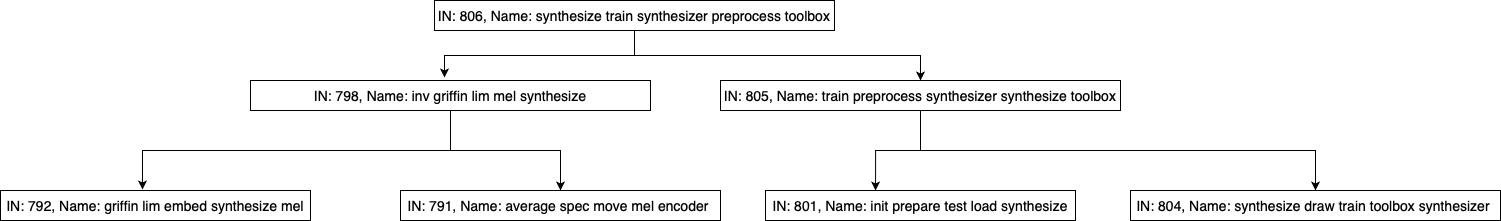
\includegraphics[width=\columnwidth]{figures/hla2/rq1_realTime1.png}
  \caption{Snippet from subject system 3 (Real-Time-Voice-Cloning)}~\label{fig:rq1_realTime1}
\end{figure*}



\subsection{ RQ2: Natural Text Summary for Abstraction Nodes}
 Natural text is more comprehensive than a few keywords. Therefore, to support abstraction nodes' comprehension in a hierarchical tree, we propose to summarize the methods' docstring in all execution paths of the node. As the number of lines in comment vary for methods,  we used only the first line of the docstring. Also, from our manual analysis, it is evident that the first line describes the function's purpose most of the time. However, for many cases, we found that docstring is absent. In those cases, we just omitted the method for generating summary. To answer our RQ2, we investigated the summary for nodes in three subject systems. 
 
 The root node 60 of subject system 1 has the text summary \textit{clustering execution paths using scipy Labeling a cluster using six variants  This function returns function name with their docstring  analyzing Python programs to build cluster tree of execution paths.} Subject system 1 is our program to cluster execution paths from a call graph. Then, we labelled the nodes in the cluster using six different techniques and also analyzed docstring to produce a summary as we discussed when introducing this research question. If we carefully observe the summary for node 60, using the TextRank algorithm, our produced summary represents very well what the first subject system does. For node 57, our approach's summary is \textit{converting tgf file to a networkX graph extracting function names from TGF file analyzing Python programs to build cluster tree of execution paths.} From the summary, we can confidently tell that abstraction node 57 deals with extracting function names from the TGF file, converting TGF format file to networkX graph.
 
 
The root node 1272 of subject system 2 (Pyan) has the summary \textit{Resolve those calls to built-in functions whose return values Return a label for this node, suitable for use in graph formats.} As Pyan deals with source code, we can see the summary saying something about resolving built-in functions and labelling nodes for graph format. We can relate this summary to the purpose of Pyan partially. For node 1271, the summary is \textit{Try to determine the full module name of a source file, by figuring out       Return the node representing the current class, or None if not inside a class definition.}
The summary for node 1271 says that the execution paths it abstracted mostly deal with determining a source file module, getting the class name a node represents. These are some standard utilities for a project which process source code. The summary for node 58 is \textit{Generate cluster figure from a dendrogram. Flattens a nested list. This function returns function name with their docstring.} Node 58 deals with plotting the dendrogram, mapping function name to docstring.

The root node 806 of subject system 3 (Real-Time-Voice-Cloning) has the summary \textit{If this function is not explicitely called, it will be run on the Args:                  Computes where to split an utterance waveform and its corresponding mel spectrogram to obtain   Derives a mel spectrogram ready to be used by the encoder from a preprocessed audio waveform.} As we have described previously, Real-Time-Voice-Cloning software can clone a voice to produce speech from text. If we see the summary generated by TextRank for node 806, we can say it deals with processing audio wave-forms. Furthermore, for node 801, the summary is \textit{Args:   Synthesizes mel spectrograms from texts and speaker embeddings.} Summary for node 801 is very small. It indicates that mostly docstring for Real-Time-Voice-Cloning is empty, and the short summary indicates text to speaker embedding, which is essential for voice cloning.

From the observation of the node summary generated by TextRank for the three subject systems, we can conclude that if functions are properly documented with docstring, this approach can complement the comprehensiveness of abstraction nodes. We faced the challenge of different formats of comments, which hampered the extraction of the docstring.  
 

\subsection{ RQ3: Effectiveness of mined patterns from execution paths}
From our manual investigation into the execution paths of an abstracted node, we find that there are recurrent patterns that can help comprehend the abstracted node. Therefore, we develop a technique to use sequential pattern mining for selecting patterns among the execution paths from those findings. 

The patterns for root node 60 of subject system 1 are

\begin{itemize}
    \item ClusteringCallGraph, python\_analysis, clustering\_using\_
    scipy
    \item ClusteringCallGraph, python\_analysis, clustering\_using
    \_scipy, labeling\_cluster
    \item ClusteringCallGraph, python\_analysis, clustering\_using\_scipy,
labeling\_cluster, tf\_idf\_score\_for\_scipy\_cluster
\end{itemize}
We can tell that node 60 works with Python code, clustering using scipy library, labelling the clusters from observing this pattern. As this is the root node of the subject system 1, we can conclude that the patterns represent the purpose.

The patterns for node 58 are 

\begin{itemize}
    \item ClusteringCallGraph, PlayingWithAST
    \item ClusteringCallGraph, get\_all\_method\_docstring\_pair\_of\_a\_project
    \item ClusteringCallGraph, get\_all\_method\_docstring\_pair\_of\_a\_project, get\_all\_py\_files
\end{itemize}
From the patterns for node 58 retrieved by sequential pattern mining, we can see it extracts docstring from all Python files, which is one of the essential parts for answering our RQ2. 

The patterns for root node 1272 are

\begin{itemize}
    \item get\_attribute
    \item resolve\_builtins, get\_attribute
    \item analyze\_binding, resolve\_builtins
\end{itemize}

From the list of patterns, we can see there is very little information. Although these patterns are for the root node, they are most frequent. Limiting the length of the minimum pattern can solve the problem. However, we can understand that getting attributes, analyzing bindings, and resolving built-ins is the most common concept for root node 1272.

The patterns for node 1240 are 
\begin{itemize}
    \item resolve\_builtins, resolve\_method\_resolution\_order, 
    C3\_linearize, C3\_merge
    \item analyze\_binding, resolve\_builtins, resolve\_method\_resolution\_
    order, C3
    \_linearize, C3\_merge
    \item resolve\_builtins, resolve\_method\_resolution\_order,
    C3\_linearize, C3\_merge, C3\_find\_good\_head, LinearizationImpossible
\end{itemize}
From the patterns of node 1240, we can see that method resolution order, linearize, resolve builtins are the main task.

The patterns for root node 806 of subject system 3 are

\begin{itemize}
    \item init, setup\_events
    \item wav\_to\_mel\_spectrogram
    \item embed\_utterance
    \item train
\end{itemize}

From the patterns for node 806, we see that it is creating different events, converting wave to spectrogram, and training model, which summarizes what Real\-Time\-Voice\-Cloning does. 
The patterns for node 804 are

\begin{itemize}
    \item wav\_to\_mel\_spectrogram
    \item encoder\_preprocess
    \item embed\_utterance
    \item encoder\_preprocess, \_preprocess\_speaker\_dirs,
    preprocess\_speaker
\end{itemize}
From the patterns of node 804, we can say that node 804 is embedding and encoding audio signals, prepossessing speaker audios.

From observing patterns of different nodes from the three subject systems, we can conclude that providing them with an abstraction node can enhance a node's comprehensibility. However, tuning the minimum length of each pattern and removing frequency-based bias should be considered to improve the patterns.


\subsection{ RQ4: Effectiveness of using label, summary and patterns together}
In RQ1, we manually analyzed how expressive the label for nodes is using word and method variants. We found that method variation of the TFIDF technique provides a more sophisticated label than its word variant, which seems ambiguous. From our analysis of RQ2, we have seen a good summary for nodes using TextRank. However, this method's success largely depends on how well the method docstring is written, excluding unrelated information is a challenge due to different formations. From RQ3, it is clear that patterns from execution paths are helpful to support nodes, although effectiveness hugely depends on selecting tuning mining pattern algorithms. Therefore, if the challenges for generating a name, summary, and patterns are solved accordingly, they will enrich the comprehension of the abstraction node, in total, the overall abstract code summary tree. 

\section{Threats to Validity}

We have picked three different subject systems of varying size so that our approach's effectiveness can be generalized to some extent. We manually analyzed the results of our techniques to reach a saturated decision. Furthermore, two of the authors of a paper submitted based on this experiment individually analyzed the findings to remove subjective biases. We carefully picked the first line skipping lines with special characters to extract the docstring for each method. 

\section{Conclusion and Future Plans}
In software engineering, program comprehension is an important research area that involves many other software maintenance tasks. Nowadays, software size and complexity are growing. To perform a maintenance task, developers need to understand how different components of the system interact. Other cognition models are studied in the literature to aid developers. Top-down and bottom-up models are popular program comprehension models. In these models, developers map high-level features with low-level implementations depending on a specific situation. Different hierarchical abstraction techniques which use call graph of dynamic and static variation exists. 

This study focused on improving a software system's abstraction hierarchically using execution paths from a static call graph. Execution paths represent low-level implementation. Grouping execution paths in a cluster tree, a software system is hierarchically abstracted. Information presented with the nodes of a cluster tree is helpful for developers to map high-level features to low-level implementations. We proposed different techniques like using word and method variant for TFIDF to label nodes, generated a summary for each node from method docstring, and mined significant patterns to attach all these three types of information with each node to aid comprehension.

To evaluate our approach, we conducted an exploratory case study to determine our proposed techniques' effectiveness. We discussed the generated output for different nodes and challenges to improve. We found that generalizing the techniques with more subject system would improve the techniques. In the future, we plan to use source code summarizing techniques \cite{wan2018improvingCodeSummary, ahmad2020transformerCodeSummary, zhu2019automaticSummaryReview} to produce a more accurate summary. Moreover, we plan to build an automated tool that, given a software system (Python), will produce an abstract code summary tree that developers can browse interactively. We have a plan to conduct a wide-scale user study to evaluate these techniques.


\chapter{Finding effectiveness of abstract code summary tree}
\section{Motivation}

\section{Approach}

\begin{algorithm}

\end{algorithm}


\section{Evaluation}

\begin{itemize}
    \item RQ1: To what extent developers agree with our approach result for getting overview of a project?
    \item RQ2: How helpful our approach to understand relevant high-level concepts targeting a low-level source code?
\end{itemize}

\section{Human-subject Study}
To evaluate the effectiveness of HCPC, we contacted with \emph{scidatamanager} development team. We have collected their source code to analyze by our system. We have invited the developers of the \emph{scidatamanager} project to validate whether HCPC can be helpful for getting overview of the \emph{scidatamanager} and accomplish a specific software maintenance task.
\subsection{Study Design}
The interview with developers are conducted remotely via Skype. The interview process was divided into four steps:
\begin{itemize}
    \item \emph{Introduction:} First, we brief each participants about our research. Then, we share our screen to show how to use HCPC tool. We demonstrate HCPC tool by exploring \emph{jupyter-client} project. We also discuss different components role to help program comprehension. Later, we asked the participants to go to a specific URL where our application is hosted and share their screen. We informed participants about two parts of the study.   
    \item \emph{Feedback on getting overview (RQ1):} In this phase, we asked the participants to explore the Cluster tree alongside different components like Node summary, Execution patterns. We requested them to check whether they can get overview of the \emph{scidatamanager} project. We encouraged the participants to express their thought while they explore different parts of the system. At the same time, we observe the participants interaction with the system and noted any feedback provided by them. When they explored the tree, we asked them whether the keywords and groups provide any reasonable clue about what the system does. Similarly, we asked them about their opinion on Node summary and Execution Patterns. We also inquired whether they have any suggestion or expectation on the components to be more helpful.
    
    
    \item \emph{Effectiveness of finding help for specific task (RQ2):} After we complete the second step, we move on to the third phase. In this step, we asked the participants to use the search option to find relevant nodes in the cluster tree and see whether they can find any help to do any specific task. We have encouraged them to remember any recent feature or issue they solved and try to see whether the HCPC tool could help them for completing the tasks. We asked the participants about how helpful Node summary, Execution patterns and the highlight of execution paths can be for someone new to the codebase to accomplish the tasks.
    \item \emph{Open discussion and closing:} At the end, we asked some open-ended questions about any suggestion and future features. The meetings lasted between 40 to 60 minutes. We ended the meeting thanking the participants for their valuable feedback and time.

\end{itemize}
\subsection{Participants and Subject System Selection}
While observing the HCPC tool output for \emph{jupyter-client} project, we can relate the different nodes content to the components in \emph{jupyter-client} documentation. We decided to conduct the study on a subject system where the team members can participate in the study to evaluate HCPC tool performance on their known codebase. We contacted the \emph{scidatamanager} team whether they could share their source code and participate in the study to evaluate HCPC. The development team of the \emph{scidatamanager} project agreed to share the codebase and participate in the study. 
\subsection{Results}
\textbf{Answering RQ1.} Participants mostly agreed that the HCPC tool can help getting overview of their project. When we asked the participants, they started to explore the abstraction tree by carefully observing the keywords for each node and expanding to child nodes. The participants agreed that high-level nodes provide hint to the features in their project. For example, participant P3 said, \emph{``I can relate to different basic components from high level nodes. If someone new joins the team, they can start from top nodes and see the path patterns for getting most frequent behaviour and then explore the code-base easily."} Participants appreciated the node summary as it states in plain text what are the purposes of the keywords in the project. Participants also find that when they see node summary for deeper nodes, the summary becomes more precise for specific features. 
According to participant P1, \emph{`` This part is helpful as it states in natural texts instead of a few words. Another interesting fact about the summary is when going deeper the summary became more precise.''} While exploring the execution patterns, we observed that participants find it helpful to know some frequent call sequences in specific nodes. However, participant P2, P3 suggested that having the frequency with the patterns would be interesting to know for understanding the importance. 

In summary, \textbf{Participants find HCPC tool helpful for getting overview of their software system with node title, summary and execution patterns.} According to their final feedback for comprehending overview, they pointed out that HCPC tool has the potential to decrease get started time for a project. According to participant P1, they believe  it can help to decrease getting started time around 50\%-60\%.

\textbf{Answering RQ2.} Participants find it useful to be able to search for specific keywords. From the interview, we observed that developers tried to highlight nodes for some recent work they have done or something they are familiar with to check how the HCPC is representing the relevant concepts. For example, participant P3 tried to highlight the nodes related to dataset publishing as it is one of the core feature of the project. While browsing the highlighted nodes and its supporting contents (node summary, execution patterns, execution paths), participant P3 identified that it is possible to know similar paths where the function is called. Another interesting observation by participant P2 is, \emph{`` I see the nodes can be searched by functions. In addition, I would love to see filters such as class, files.''} Participant P3 shared from their previous experience that sometimes they have to fix some issues of another project which not very well documented and they struggle a lot to figure out the abstraction patterns followed in the codebase. Both participant P3, P1 suggested using the search option to explore execution paths will be helpful to decrease time required for completing tasks in those scenarios. Another interesting observation from the interview is for some searches multiple nodes are highlighted which shows the specific functions being used in different scenarios. We observed participants was enthusiastic to know what are the different directions the function is being used by going deeper in the abstraction tree. In addition, participant P1 shared that many times they try to search the codebase with some keywords using the find option provided by the editor to retrieve relevant files. However, the search result does not show any order or how these class or methods are being called. They suggested that with the execution patterns and paths HCPC can help replacing the raw find workflow into more execution based search process. In summary, \textbf{the feedback from the participants and our observation during the interview it is viable that the search option of  HCPC has the potential to help in day-to-day software maintenance activities. } 

% To Do using find button for searching which do not have any order

During our open-ended questions and suggestions, we found valuable feedback for future development and adaptation of the HCPC tool. One important suggestion is to incorporate automatic comment generation techniques for methods which have no comments. This will be a valuable future work suggestion for our HCPC tool, as it will be helpful for projects which do not follow best practices. Another worth mentioning future work is suggested by participant P2 is to generate report of the abstraction structure where developers can edit the components name according to their understanding from the HCPC tool. These report can be used as a documentation of the project structure from static execution perspective. In addition, participants suggested to enable the option to export projects from GitHub which will be useful for quickly exploring a new codebase. From the above discussion, \textbf{we can conclude that HCPC tool can help to get overview of a software project from static execution perspective and can be used to help doing a specific task in hand.}


% TODO
% github, report generation 


\subsection{Threats to validity}



\section{Implementation }
In this section, we briefly highlight different parts of our implementation as shown in Figure \ref{fig:architecture}.

\begin{enumerate}
    \item We clone the source code from GitHub in a temporary folder. The source code will be used in the next phase by Python static code analyzer.
    \item We use Pyan~\cite{pyan} as static Python code analyzer. Pyan goes through all the \emph{*.py} files looking for which method calls which method. Pyan generates a text file  which encodes all the methods with numbers and then contains which method calls which method. We generate static call graph using NetworkX~\cite{networkx} with the caller-callee relationships generated by Pyan.
    
\begin{figure*}[h]
\centering
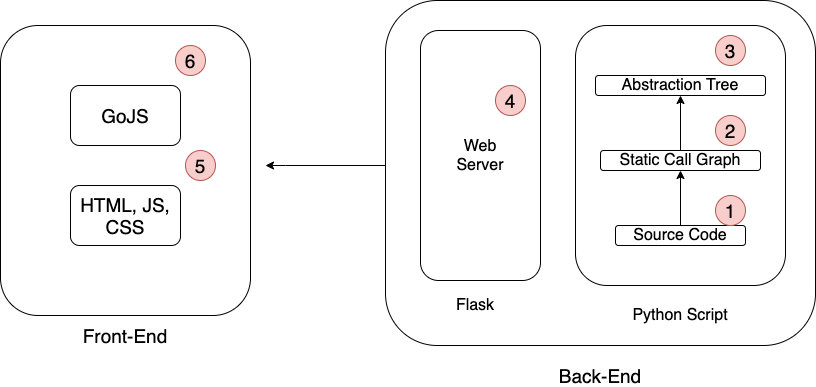
\includegraphics[width=\columnwidth]{figures/hla3/hla3_implementation.png}
\caption{Architecture of HCPC tool }~\label{fig:architecture}
\end{figure*}

    \item We generate execution paths from the call graph created in previous step.
Execution paths are grouped using Agglomerative Hierarchical Clustering~(AHC) algorithm provided by Scipy~\cite{scipy} library with \emph{ward} method as distance metric. We have a binary tree structure where leaf nodes are execution paths and other nodes are clusters at different levels. We call these cluster nodes as abstraction nodes. The abstraction nodes have collection of execution paths. For each abstraction node, we generate three properties. For each node, we create node title by applying information retrieval techniques ( Scikit-learn~\cite{scikit-learn} for TFIDF and Gensim~\cite{gensim} for LDA, LSI ) on the method names of all execution paths of a node. Then we produce node summary by summarizing (TextRank by Gensim) method comments of all the execution paths of the node. Last we generate execution patterns by pattern mining among the execution paths of the node~(PrefixSpan \cite{prefixspan}). We write all the node data in a text file named with the project name. Data is written in JSON format where each node is keyed with their ID and they have parent\_id, node title, node summary, execution patterns and execution paths associated with them. 
    \item We have Flask server for interacting with front-end. Client requests which subject system they want to explore and the server returns JSON response with the abstraction tree. 
    \item For the interface of our web application, we have used HTML, CSS, and JQuery. When a specific node is right-clicked, detail information about the node is filled to the node details panel.
    \item We used GoJS for building the abstraction tree diagram. Each abstraction  is a GoJS node and different properties of the abstraction nodes are binded to GoJS nodes. 

\end{enumerate}


\section{Interface}

In this section, we will discuss the different components of our HCPC tool shown in Figure \ref{fig:interface}.

\begin{itemize}
    \item \textbf{Abstract Tree Panel(A).} In the panel, the main abstraction tree is presented. The root nodes are presented vertically which can be possible to expand with their child nodes. By right clicking the mouse on a node will load different information of the abstraction node in the right side of the interface.
    \item \textbf{Number of execution paths(B).} As each node in the abstraction tree are a collection of execution paths, we show the number of execution paths for a selected node in this element.
    \item \textbf{Files (C).} In the element, we show the unique files of all the methods of the execution paths belong to.
    \item \textbf{Node summary (D).} In the element, we have provided natural text description of a node. When developers select a node, the text description of the node will appear in the element. 
    \item \textbf{Execution Patterns (E).} In the element, for a selected abstraction node, frequent function call patterns are presented with the file they are associated with. In the current setting, top-10 frequent execution patterns are shown. 
    
    \item \textbf{Execution paths (F).} In the element, we show five execution paths of a selected abstraction node. The execution paths complement the execution patterns by showing a glimpse of the real execution paths. Moreover, when a specific method is searched, the execution paths with the searched method is presented instead first five methods.
    
    \item \textbf{ Node label technique and search panel (G).} The panel has three drop-down boxes. First, developers can select which subject system they want to explore. Second, they can choose which technique to be used for labeling the nodes in abstraction tree. Third, this drop-down box is search enabled and it helps to highlight the nodes which have the searched method in their execution paths.
\end{itemize}

\begin{figure*}[h]
  \centering
  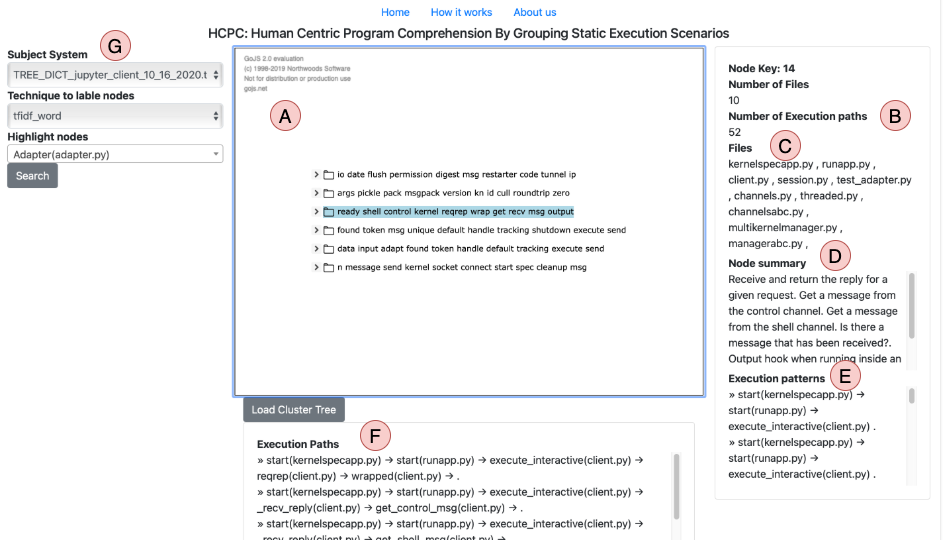
\includegraphics[width=\columnwidth]{figures/hla3/hla3_interface.png}
  \caption{HCPC tool interface }~\label{fig:interface}
\end{figure*}


\section{Guide to use HCPC}
The tool can be used in two ways. First, a developer new to the code-base can load the abstraction tree which start with the root node. In the right side panel, for each node the number of execution paths, a brief natural text summary, and few frequent execution patterns are presented. Therefore, the developer can start first by observing summary, patterns of the root node. Now, the child nodes of the root node can be expanded and  similarly explored by observing corresponding node summary and patterns. The developer can continue this way according to their need to get acquainted with the coda-base behavior and high-level concepts in the code-base.

Second, a new contributor to a open source project can utilize the tool to understand high-level concepts related to a specific method. Developers first start from looking to open issues of a repository to find something work on. The issues are natural text description which provides information regarding a bug or a feature enhancement request. Developers can identify few keywords and use our tool to find matching methods relevant to the keywords. Next, a specific method can be selected to highlight relevant nodes in the tree. The difference between the first approach here is developers will be able to browse the tree with focus to the selected method. The node titles relevant to selected method will be highlighted so that the developer can expand their child nodes. By this way, the developer can start from the high-level concept to low-level source code related concepts for a specific method. By iterating this process, the developer can grasp high-level domain knowledge (with comment summary and IR techniques on function names) alongside insight into program execution scenarios which decreases the overhead due to lack of domain knowledge in the code-base. 

\section{Graphical demo of the tool} 
We have picked \emph{jupyter-client}\footnote{https://github.com/jupyter/jupyter\_client} as the subject system to show how the tool can be used following the two above mentioned techniques. To discuss the effectiveness of our tool using \emph{jupyter-client}, first we will discuss high level functionalities of \emph{jupyter-client} from their documentation. Later, we will present the information provided by our tool and discuss whether our tool provides similar or more information to comprehend the \emph{jupyter-client} project. \emph{jupyter-client} has three components. First, \emph{kernelspec} deals with specify different type of kernels from predefined files. Second, kernel manager which is responsible for start, stop and signaling kernels for different scenarios. Third, kernel client which is responsible for communicating with kernels for code execution and other tasks \footnote{https://jupyter-client.readthedocs.io/en/stable/index.html}. From the above components we can get an abstract idea of the features of \emph{jupyter-client}. Now, we will discuss the high-level features suggested by HCPC tool. Below we have listed few high-level features of the \emph{jupyter-client} project. The features are found by expanding the tree to three depth. More specific features are possible to get by diving deep into the tree.

\begin{figure*}[h]
  \centering
  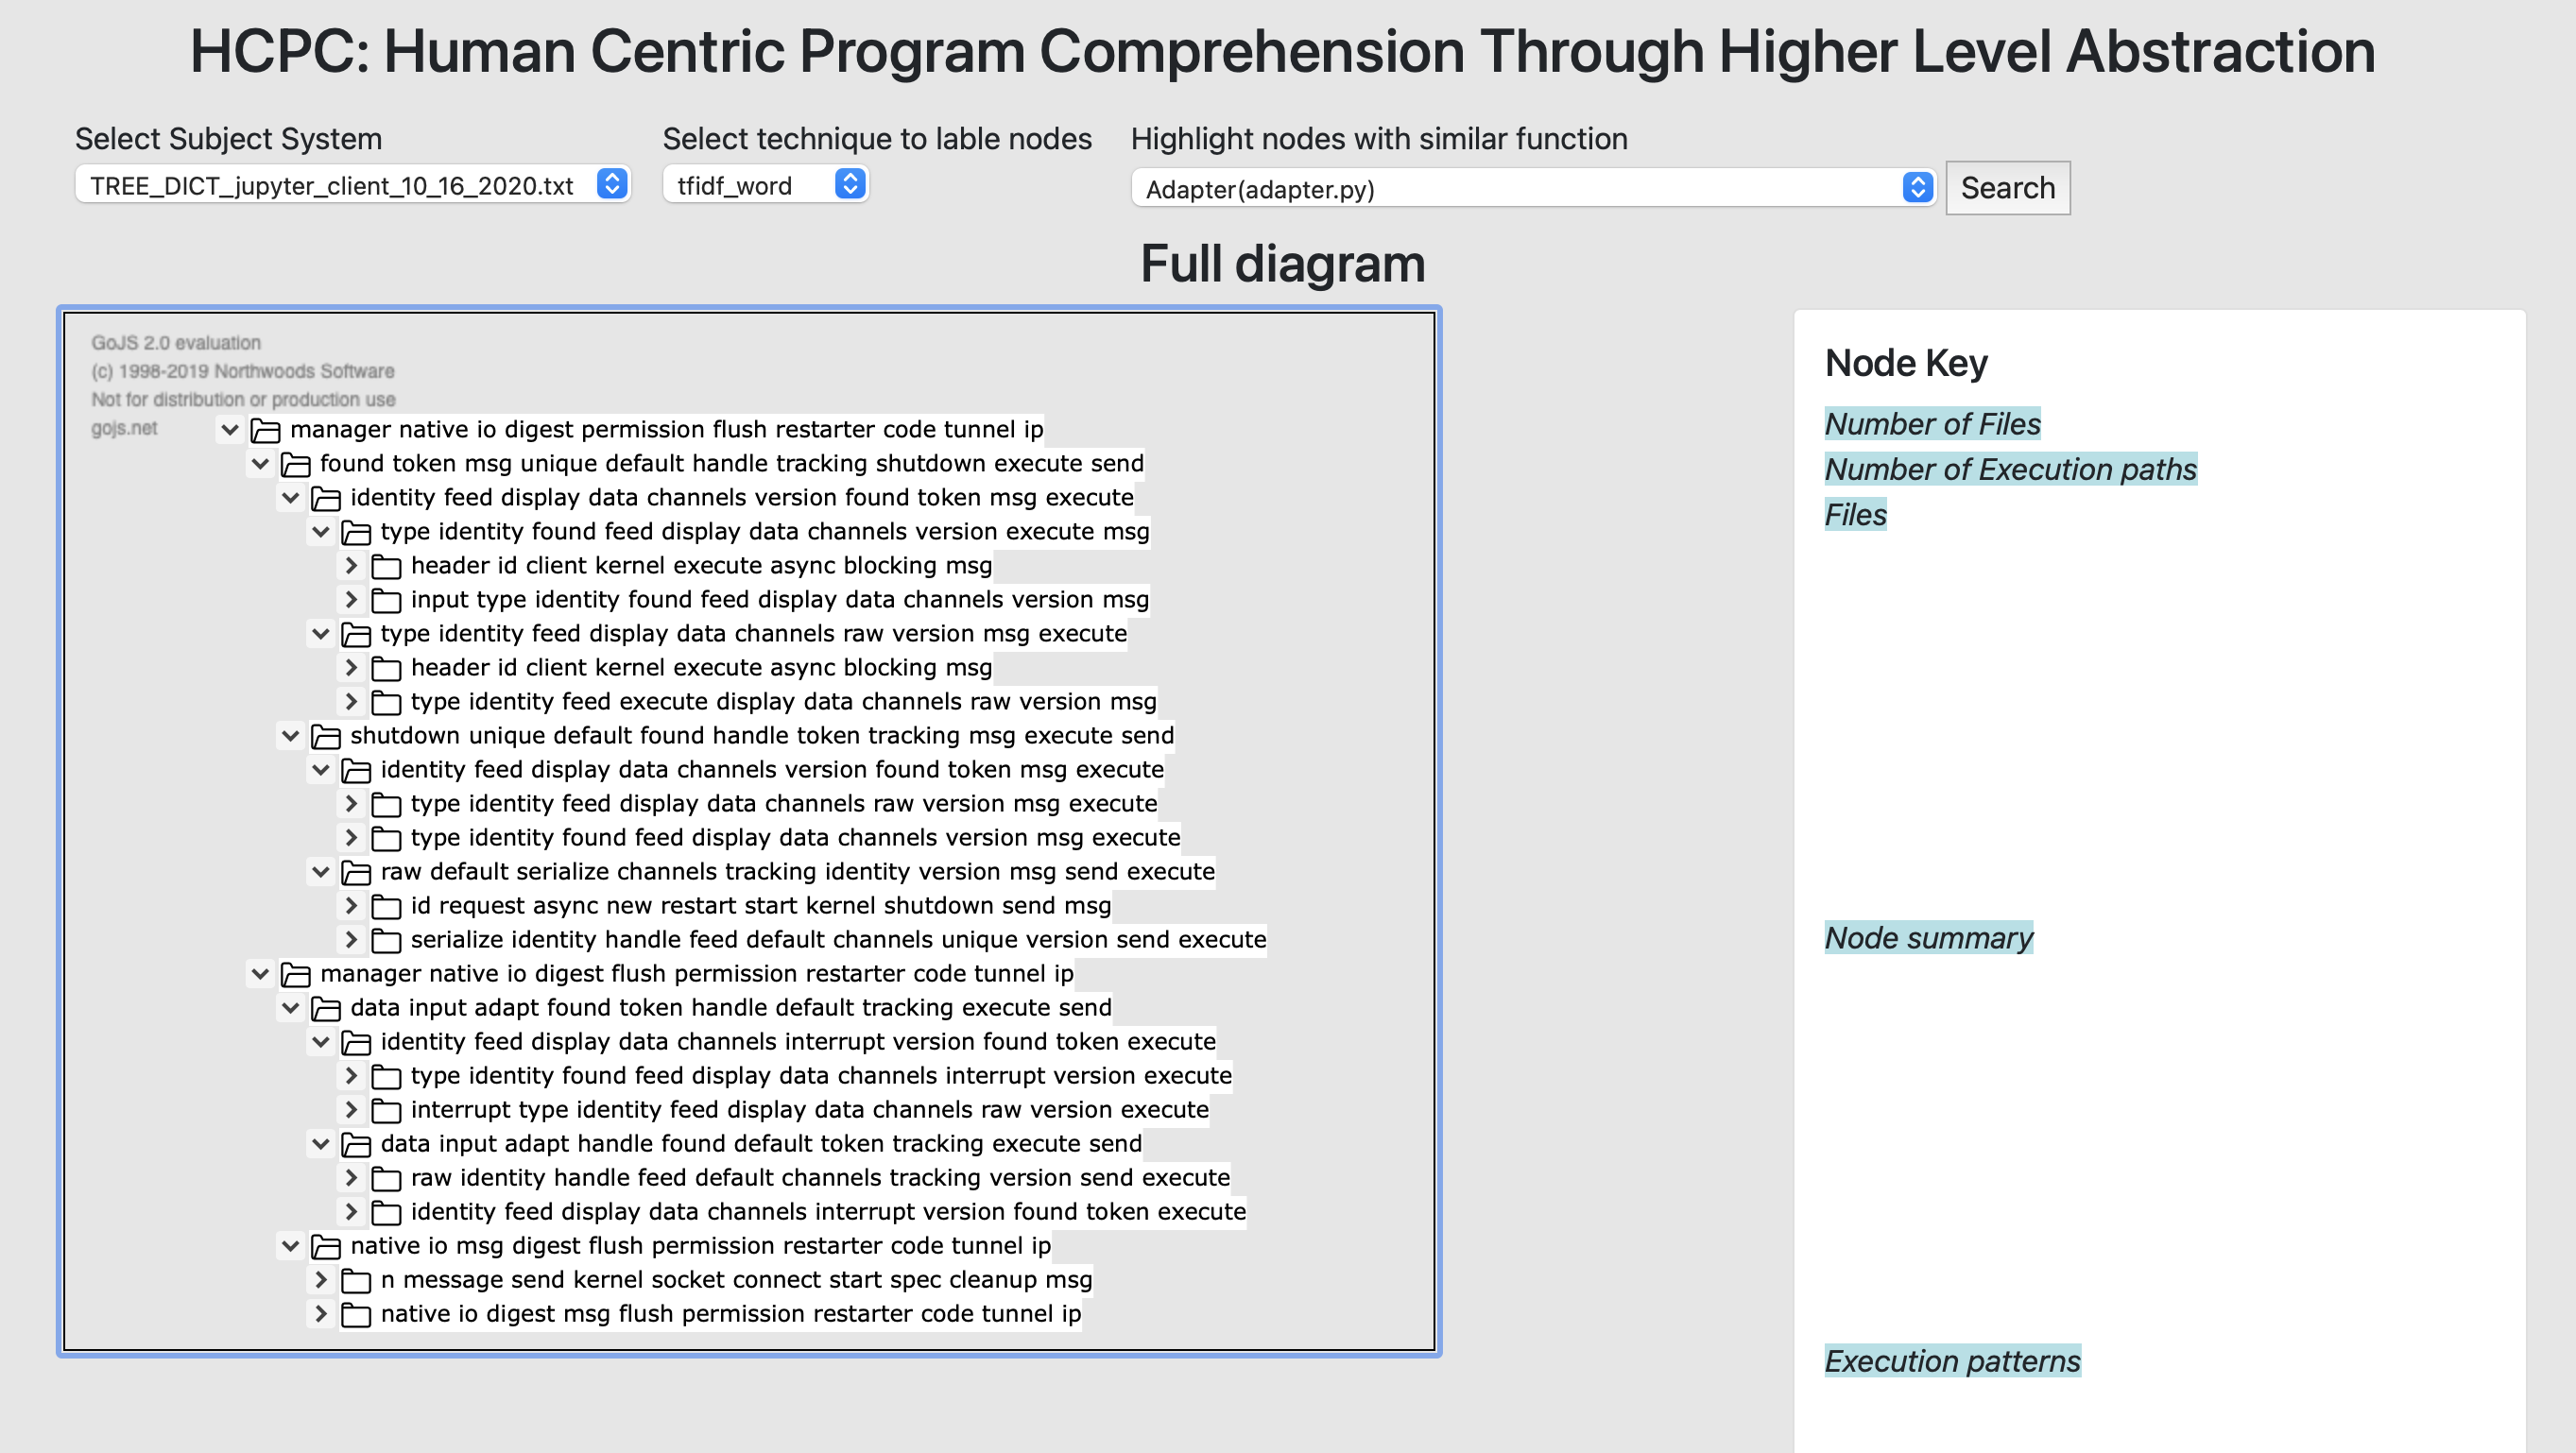
\includegraphics[width=\columnwidth]{figures/hla3/tool_overview_jupyter.png}
  \caption{HCPC tool overview for jupyter\_client project }~\label{fig:tool_overview_jupyter_client}
\end{figure*}

\begin{itemize}
    \item Request kernel info. Request comm info. Tab complete text in the kernel's namespace. Get metadata information about an object in the kernel's namespace. Ask the kernel whether some code is complete and ready to execute.
    \item Forgets randomly assigned port numbers and cleans up the connection file. Restarts a kernel with the arguments that were used to launch it. Write connection info to JSON dict in self.connection\_file. Restarts a kernel with the arguments that were used to launch it.
    \item Request kernel info. Given a message or header, return the header. Request comm info. Tab complete text in the kernel's namespace. wrapper for doing common steps for validating an execution request. Pass a message to the ZMQ socket to send. message format.
    \item Send a shutdown request via control channel. Attempts to stop the kernel process cleanly. Restarts a kernel with the arguments that were used to launch it.
\end{itemize}

From the above text blocks, we can understand that \emph{jupyter-client} is relevant to working with kernels, it uses ZMQ socket to communicate with kernels, and work with kernel information. 

Next, it is possible to browse the tree by focusing on a specific method. In figure \ref{fig:tool_shutdown_all}, we can see the nodes in the tree are marked to indicate they are relevant to shutdown\_all method. Developers can investigate the nodes marked to understand relevant features of shutdown\_all method. 

\begin{figure*}[h]
  \centering
  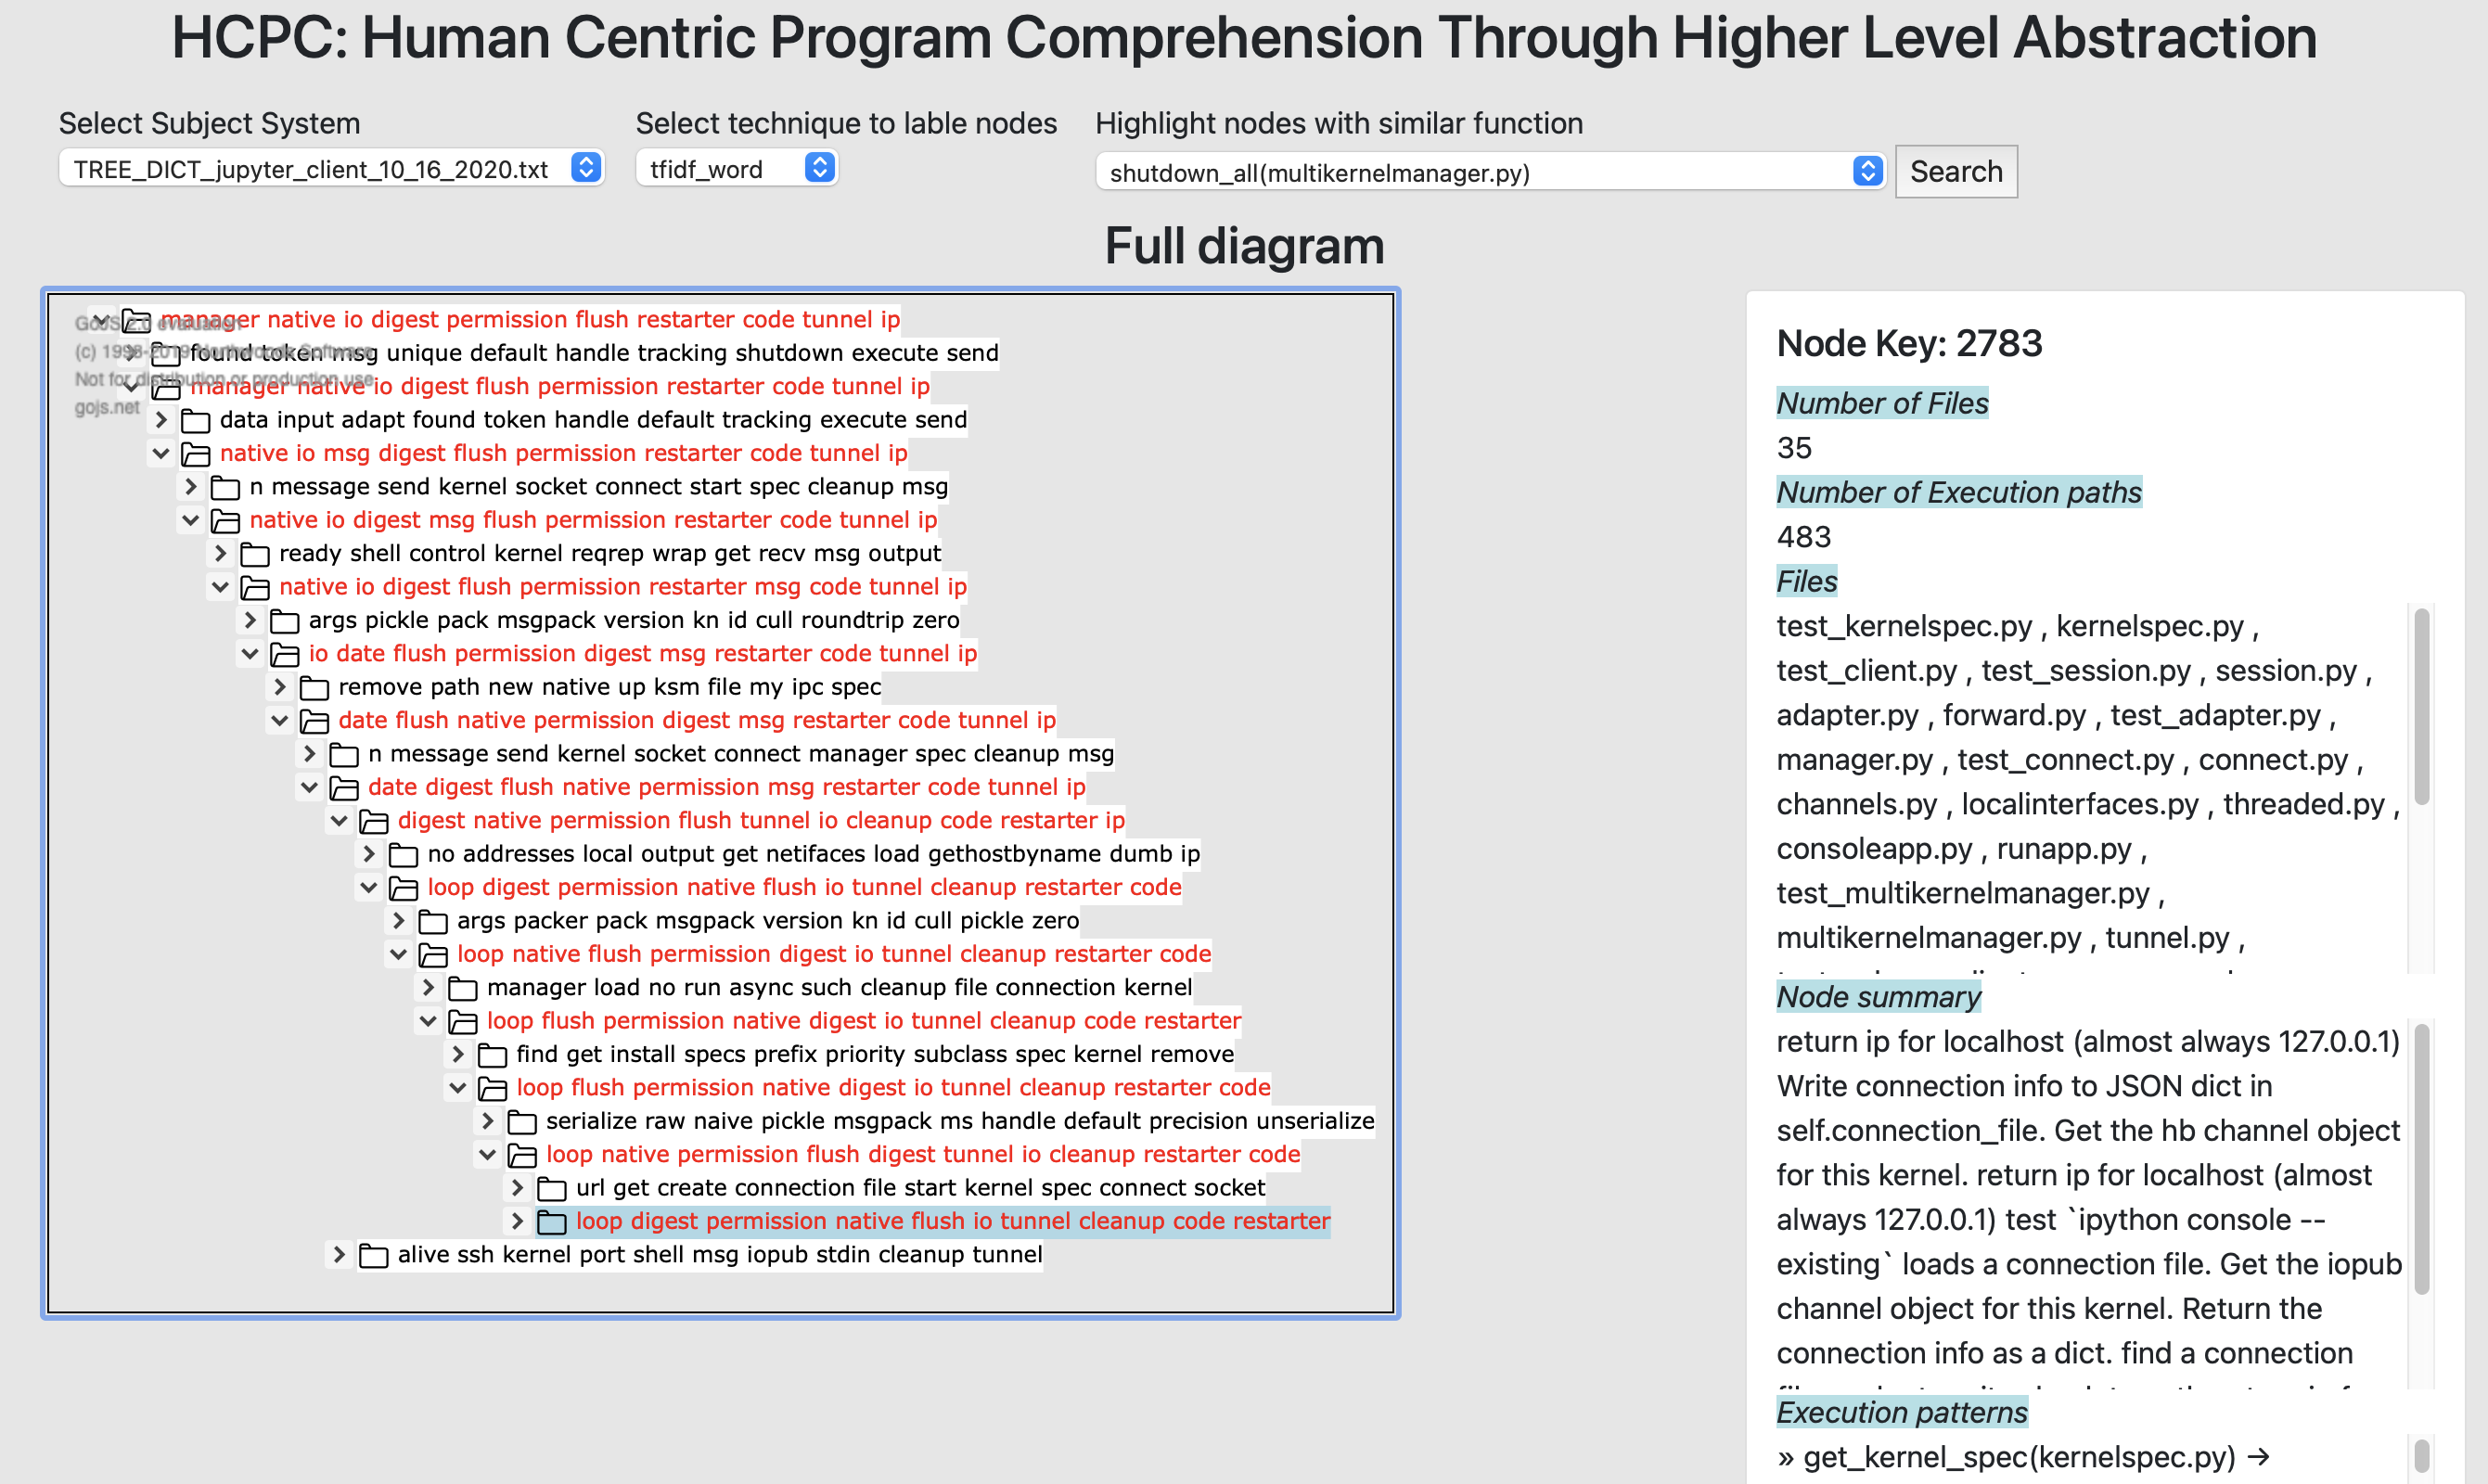
\includegraphics[width=\columnwidth]{figures/hla3/tool_shutdown_all.png}
  \caption{HCPC tool when focusing to find features related to shutdown\_all method }~\label{fig:tool_shutdown_all}
\end{figure*}


\begin{itemize}
    \item check that a kernel id is valid. Interrupts the kernel by sending it a signal. Wait for kernel shutdown, then kill process if it doesn't shutdown. Shutdown all kernels. Sends a signal to the process group of the kernel (this. Restarts a kernel with the arguments that were used to launch it. Attempts to stop the kernel process cleanly. Get the single KernelManager object for a kernel by its uuid.
    \item Get the hb channel object for this kernel. Get the stdin channel object for this kernel. Stops all the running channels for this kernel. Get the iopub channel object for this kernel. Get the control channel object for this kernel. Get the shell channel object for this kernel.
    
\end{itemize}

From above information provided by the tool, we can know how the shutdown\_all method works. Also we know that kernel object has different kind of channels for communication such as iopub, stdin.  

\section{Conclusion}


\chapter{Conclusion and Future Plan}
\label{chapter:conclusion}
In this thesis, we have worked on grouping execution paths of a software project for helping developers comprehend the codebase faster and locate related concepts for their tasks in hand. We start with existing works on clustering static execution paths for presenting high-level features in a software project. However, we find some limitations and scope of improvement to make the abstract code summary more usable for the daily activities of software developers. First, we experimented with different information retrieval techniques to find out which techniques provide more helpful labels for abstraction nodes. We also proposed using the terms in method names instead of whole method name as input for IR techniques. We also conducted a human subject study to find out how developers rate different IR techniques and compared automatic naming with manual naming by developers. From the study, we found TFIDF with terms in method are better supported by the manual labeling compared to LDA, LSI techniques. Moreover, developers preferred the words variant than the method variant of the labeling technique. Second, we proposed to add additional information such as node summary, execution patterns for each abstraction node to make the abstract code summary tree more comprehensible. We conducted a case study with three different subject systems to find the potential of attaching the two new information for each abstraction node. We found that attaching node summary, and execution patterns can complement node labels for more detailed understanding in relation to source code. However, we observed that using an agglomerative cluster tree poses some difficulty to browse as it presents all the clustering step by step. In addition, we noticed that it is difficult to explore the tree when targeting some specific keywords. In our third study, we addressed the issue of abstraction tree being overwhelming to browse by simplifying the agglomerative cluster tree using cluster flattening technique. Additionally, we have added an abstraction node highlighting technique for browsing the tree targeting specific keywords or methods. To evaluate the usefulness of our technique, we developed a web application called the HCPC. We performed a human subject study with an industry project and their developers. From the study, we found that the HCPC tool can help developers get started with a project alongside finding relevant execution patterns for specific tasks in hand.

In future, we plan to adopt automatic method summarizing techniques~\cite{wan2018improvingCodeSummary, ahmad2020transformerCodeSummary, zhu2019automaticSummaryReview} since in industry settings not every method is properly documented. We also plan to incorporate the GitHub project import option for exploring in the HCPC tool. Moreover, we will add feature to export reports with our analysis result. We have a plan to conduct a wide-scale user study with popular Python open-source projects.


%%%%%%%%%%%%%%%%%%%%%%%%%%%%%%%%%%%%%%%%%%%%%%%%%%%%%%%%%%%%%%%%
% The Bibliograpy should go here. BEFORE appendices!
%%%%%%%%%%%%%%%%%%%%%%%%%%%%%%%%%%%%%%%%%%%%%%%%%%%%%%%%%%%%%%%%


% Typeset the Bibliography.  The bibliography style used is "plain".
% Optionally, you can specify the bibliography style to use:
% \uofsbibliography[stylename]{yourbibfile}

\uofsbibliography{reference}

% If you are not using bibtex, comment the line above and uncomment
% the line below.  
%Follow the line below with a thebibliography environmentand bibitems.  
% Note: use of bibtex is usually the preferred method.

%\uofsbibliographynobibtex


%%%%%%%%%%%%%%%%%%%%%%%%%%%%%%%%%%%%%%%%%%%%%%%%%%%%%%%%%%%%%%%%%%%%%%%%%
% APPENDICES
%
% Any chapters appearing after the \appendix command get numbered with
% capital letters starting with appendix 'A'.
% New chapters from here on will be called 'Appendix A', 'Appendix B'
% as opposed to 'Chapter 1', 'Chapter 2', etc.
%%%%%%%%%%%%%%%%%%%%%%%%%%%%%%%%%%%%%%%%%%%%%%%%%%%%%%%%%%%%%%%%%%%%%%%%%%

% Activate thesis appendix mode.
\uofsappendix

% Put appendix chapters in the appendices environment so that they appear correcty
% in the table of contents.  You can use \input's here as well.
\begin{appendices}

\chapter{Simple Calculator program to demonstrate the clustering approach}
\label{appendix:calculator}

\lstinputlisting{appendix/calculator.py}

\end{appendices}

\end{document}
